 %% This is file `elsarticle-template-3-num.tex',
%%
%% Copyright 2009 Elsevier Ltd
%%
%% This file is part of the 'Elsarticle Bundle'.
%% ---------------------------------------------
%%
%% It may be distributed under the conditions of the LaTeX Project Public
%% License, either version 1.2 of this license or (at your option) any
%% later version.  The latest version of this license is in
%%    http://www.latex-project.org/lppl.txt
%% and version 1.2 or later is part of all distributions of LaTeX
%% version 1999/12/01 or later.
%%
%% The list of all files belonging to the 'Elsarticle Bundle' is
%% given in the file `manifest.txt'.
%%
%% Template article for Elsevier's document class `elsarticle'
%% with numbered style bibliographic references
%%
%% $Id: elsarticle-template-3-num.tex 165 2009-10-08 07:58:10Z rishi $
%% $URL: http://lenova.river-valley.com/svn/elsbst/trunk/elsarticle-template-3-num.tex $
%%

\documentclass[times,3p]{elsarticle}

%% Use the option review to obtain double line spacing
%% \documentclass[preprint,review,12pt]{elsarticle}

%% Use the options 1p,twocolumn; 3p; 3p,twocolumn; 5p; or 5p,twocolumn
%% for a journal layout:
%% \documentclass[final,1p,times]{elsarticle}
%% \documentclass[final,1p,times,twocolumn]{elsarticle}
%% \documentclass[final,3p,times]{elsarticle}
%% \documentclass[final,3p,times,twocolumn]{elsarticle}
%% \documentclass[final,5p,times]{elsarticle}
%% \documentclass[final,5p,times,twocolumn]{elsarticle}

%% PACKAGES

%% if you use PostScript figures in your article
%% use the graphics package for simple commands
%% \usepackage{graphics}
%% or use the graphicx package for more complicated commands
\usepackage{graphicx}
%% or use the epsfig package if you prefer to use the old commands
%% \usepackage{epsfig}

%% The amssymb package provides various useful mathematical symbols
\usepackage{amssymb}
%% The amsthm package provides extended theorem environments
%% \usepackage{amsthm}

%% The numcompress package shorten the last page in references.
%% `nodots' option removes dots from firstnames in references.
%% `nocompress' option prevent shortening of last page as
%% by default it will shorten.

\usepackage[nodots]{numcompress}
%% The lineno packages adds line numbers. Start line numbering with
%% \begin{linenumbers}, end it with \end{linenumbers}. Or switch it on
%% for the whole article with \linenumbers after \end{frontmatter}.
%% \usepackage{lineno}

%% natbib.sty is loaded by default. However, natbib options can be
%% provided with \biboptions{...} command. Following options are
%% valid:

%%   round  -  round parentheses are used (default)
%%   square -  square brackets are used   [option]
%%   curly  -  curly braces are used      {option}
%%   angle  -  angle brackets are used    <option>
%%   semicolon  -  multiple citations separated by semi-colon
%%   colon  - same as semicolon, an earlier confusion
%%   comma  -  separated by comma
%%   numbers-  selects numerical citations
%%   super  -  numerical citations as superscripts
%%   sort   -  sorts multiple citations according to order in ref. list
%%   sort&compress   -  like sort, but also compresses numerical citations
%%   compress - compresses without sorting

\usepackage{lineno}

%\usepackage{fleqn}
\usepackage{tikz}
\usepackage{pgfplots}
\usepackage{booktabs}
\usepackage{multirow}
\usepackage{amsmath}
\usepackage{nomencl}
\usepackage{framed} % Framing content
\usepackage{multicol} % Multiple columns environment
\usepackage{float}
\usepackage{rotating}

\usepackage[pdftex,bookmarks=true]{hyperref}
\hypersetup{ 
    colorlinks,% 
    citecolor=black,% 
    filecolor=black,% 
    linkcolor=black,% 
    urlcolor=black,
		pdfstartview=FitH
} 

\biboptions{square,sort&compress}

%% Contraction of references
\makeatletter
\def\NAT@spacechar{}
\makeatother

\renewcommand*\nompreamble{\begin{multicols}{2}}
\renewcommand*\nompostamble{\end{multicols}}

\RequirePackage{ifthen}

\renewcommand{\nomgroup}[1]{%
\ifthenelse{\equal{#1}{0}}{\item[\emph{Symbols}]}{
\ifthenelse{\equal{#1}{S}}{\item[\emph{Subscripts}]}{}}
\ifthenelse{\equal{#1}{P}}{\item[\emph{Superscripts}]}{
\ifthenelse{\equal{#1}{A}}{\item[\emph{Abbreviations}]}{}}
\ifthenelse{\equal{#1}{G}}{\item[\emph{Greek letters}]}{
\ifthenelse{\equal{#1}{O}}{\item[\emph{Others}]}}
}

\makeindex
\makenomenclature

\journal{Energy}

\makeatletter
\def\ps@pprintTitle{%
 \let\@oddhead\@empty
 \let\@evenhead\@empty
 \def\@oddfoot{}%
 \let\@evenfoot\@oddfoot}
\makeatother

\begin{document}

\begin{frontmatter}

\title{Exergetic efficiency definitions for oil and gas platforms}

\author[dtu]{Tuong-Van Nguyen\corref{cor}} \cortext[cor]{Principal corresponding author. Tel.: +45 4525 4129} \ead{tungu@mek.dtu.dk}
\author[ntnu1]{Mari Voldsund} \ead{mari.voldsund@ntnu.no}
\author[dtu]{Brian Elmegaard} \ead{be@mek.dtu.dk}
\author[ntnu2]{Ivar St\aa le Ertesv\aa g}  \ead{ivar.s.ertesvag@ntnu.no}

\address[dtu]{Section of Thermal Energy, Department of Mechanical Engineering, Technical University of Denmark,\\ Building 403, Nils Koppels All\'{e}, 2800 Kongens Lyngby, Denmark}
\address[ntnu1]{Department of Chemistry, Norwegian University of Science and Technology, \\ H\o gskoleringen 5, 7491 Trondheim, Norway}
\address[ntnu2]{Department of Energy and Process Engineering, Norwegian University of Science and Technology, \\ Kolbj\o rn Hejes vei 1b., 7491 Trondheim, Norway}

\begin{abstract}

Exergy-based efficiencies are a measure of the thermodynamic perfection of systems and processes: they can be expressed for any plant for which the inputs and outputs are expressible in terms of exergy. However, an exact formulation of this criterion for oil and gas platforms is made difficult by the great differences in working conditions, design setups and operating strategies amongst them. In this paper, possible interpretations of exergetic efficiencies for these specific systems are presented and discussed. We assessed and compared several formulations of exergetic efficiencies introduced in the literature for relatively similar processes. They were then applied to four real-case studies of the North Sea region and their relevance was evaluated. The `input-output' exergy efficiency was above 98\% in all cases while the corresponding figures for the `consumed-produced' exergy efficiency were between 10\% and 75\%, depending on the considerations on the `consumed' and `produced' exergies and on the case study. 

\end{abstract}

\begin{keyword}
Exergy \sep Efficiency \sep Oil and gas platforms
\end{keyword}

\end{frontmatter}

%
%% Start line numbering here if you want
%%
%\linenumbers

%% Main Text

%%%%%%%%% NOMENCLATURE %%%%%%%%%

\begin{table*}[!t]
  \begin{framed}
  \scriptsize
    \printnomenclature
  \end{framed}
\end{table*}

%%%%%%%%% CONTENTS %%%%%%%%%


\tableofcontents




%%%%%%%%% MAIN PART %%%%%%%%%


%%%%%%%%% SECTION: INTRODUCTION %%%%%%%%%

\section{Introduction}
\label{sec:introduction}
	


Conventional indicators for evaluating the performance of oil and gas platforms, such as the power consumption per unit of oil equivalent produced, or the amount of carbon dioxide produced per unit of oil equivalent, present inherent limitations. Each oil field has different natural characteristics (e.g. gas-to-oil ratio, well-fluid composition, field size) and comparing different facilities with these metrics could be misleading. They provide useful information on the energy use of the onsite processes, but they cannot be used alone to compare the performance of different facilities \cite{Svalheim2002,Svalheim2003}.

Exergy Analysis is a quantitative assessment method that is based on both the First and Second Laws of Thermodynamics. This thermodynamic method presents advantages over a conventional energy analysis: it pinpoints the locations and types of the irreversibilities taking place within a given system. As emphasised by Rivero \cite{Rivero2002}, the application of the exergy concept in the petroleum industry would provide more detailed and consistent information on the performance of petrochemical systems. The exergy concept was introduced in the literature along with the concept of exergetic efficiency, which aims at measuring the degree of thermodynamic perfection of the process under investigation.  

Formulations of exergy-based criteria of performance have been proposed from the middle of the 20$^{th}$ century, with, amongst others, the contributions of Nesselmann \cite{Nesselmann1952} and Fratzscher \cite{Fratzscher1981,Fratzscher1986}. Both works reported the definition of the exergetic efficiency of a given system as the ratio of its total exergy output to its total exergy input and discussed the advantages and drawbacks of such formulation. Grassmann \cite{Grassmann1950} and Nesselmann \cite{Nesselmann1953} suggested to define the exergetic efficiency as the ratio of the part of the exergy transfers that contribute to the transformations taking place, i.e. \emph{`consumed'} exergy, to the part of the exergy transfers that are generated within the system, i.e. \emph{`produced'} exergy. Based on these works, Baehr \cite{Baehr1965,Baehr1968} proposed his own expressions for these two terms. He also stressed the difficulty of providing a non-ambiguous definition of an exergetic efficiency, as different views on \emph{`consumed'} and \emph{`produced'} exergies may apply.

Further advances within this field include the studies of Brodyansky \cite{Brodyansky1994}, Szargut \cite{Szargut1988,Morris1994,Szargut1998}, Kotas \cite{Kotas1995} and Tsatsaronis \cite{Tsatsaronis1993,Thermoeconomics2001}. Brodyansky \cite{Brodyansky1994} suggested a systematic procedure for calculating the \emph{`produced'} and \emph{`consumed'} exergies, without regarding whether they are useful to the owner of the system. His work was based on the concept of \emph{`transit exergy'} introduced by Kostenko \cite{Kostenko1983} and discussed also in Sorin et al. \cite{Sorin1994}. Szargut \cite{Szargut1988,Morris1994,Szargut1998}, Kotas \cite{Kotas1995} and Tsatsaronis \cite{Tsatsaronis1993,Thermoeconomics2001} proposed to consider only the exergy transfers representing the \emph{`desired'} exergetic output and the \emph{`driving'} exergetic input of the system, leading to the concept of  \emph{`product'} and \emph{`fuel'} exergies. Such considerations must be consistent with the purpose of owning and operating the system of investigation \cite{Kotas1980,Kotas1980a,BejanAdrian;TsatsaronisGeorge;Moran1996,Moran1998}, both from an economic and a thermodynamic prospect. Lazzaretto and Tsatsaronis \cite{Lazzaretto1999,Lazzaretto2006} suggested a systematic procedure for defining the exergetic efficiency at a component level. However, at a process level, a unique formulation may not be available and several expressions may be appropriate \cite{Tsatsaronis1993}.

Various expressions of exergetic efficiency for separation systems have been illustrated in the literature and different considerations have applied \cite{Brodyansky1994,Kotas1995,Tsatsaronis1993,Sorin1994a}. Cornelissen \cite{Cornelissen1997} investigated three of the proposed formulations for an Air Separation Unit (ASU) and a Crude Distillation Plant (CDP). Different values were obtained, illustrating the variations and lack of uniformity across the exergetic efficiency definitions \cite{Baehr1965,Baehr1968,Lior2007}. However, the only studies dealing exclusively with oil or gas processing plants are the works of Oliveira and Van Hombeeck \cite{Oliveira1997}, Voldsund et al. \cite{Voldsund2010,Voldsund2012}, and Rian and Ertesv\aa g \cite{Rian2012}, who proposed their own interpretations of \emph{`product'} and \emph{`fuel'} exergies.

The literature seems to contain little, if none, on (i) a uniform performance parameter for oil and gas installations, (ii) the application of the exergetic efficiency concept, and on (iii) the comparison of the different definitions. This study is aimed at addressing these gaps and is part of two broader projects conducted at the Norwegian University of Science and Technology (NTNU) and at the Technical University of Denmark (DTU). Four main steps were required in the present study:
\begin{itemize}
	\item derivation and formulation of exergetic efficiencies for offshore platforms;
	\item modelling and simulation of four oil and gas facilities in the North Sea region; \textbf{(remove this one? belongs to paper 2...)}
	\item application of the different expressions;
	\item analysis of their sensitivity to changes in design and operating conditions.
\end{itemize}

This paper is structured as follows: Section \ref{sec:system_description} presents the oil and gas platforms investigated in this study and Section \ref{sec:background} describes the theoretical background. Section \ref{sec:efficiency} reports the derived definitions of exergetic efficiencies, while Section \ref{sec:comparison} illustrates the comparison of the four oil and gas facilities. The pertinence of the different exergetic efficiency formulations is discussed in Section \ref{sec:discussion} and concluding remarks are outlined in Section \ref{sec:conclusion}.


\section{System description}
\label{sec:system_description}

\subsection{General overview}
\label{subsec:overview}

Offshore platforms are large structures with facilities to extract and process petroleum from subsea reservoirs. Petroleum is processed in a processing plant using power (and often also heat) that is produced in a utility plant. The power is produced by gas turbines fuelled with a fraction of produced gas, or, alternatively, heavy oil or diesel. A heating demand is either met by using fuel gas burners, electric heaters or by indirect waste heat recovery. 

In this work we distinguish between three different control volumes: the processing plant, the utility plant and the overall plant (which is the combination of the processing plant and the utility plant). The drilling- and accomodation parts are not included in the study. The control volumes with the in- and outgoing material- and energy streams are shown schematically in Figure~\ref{fig:control_volume}. 

\begin{figure*}[htbp]
	\centering
	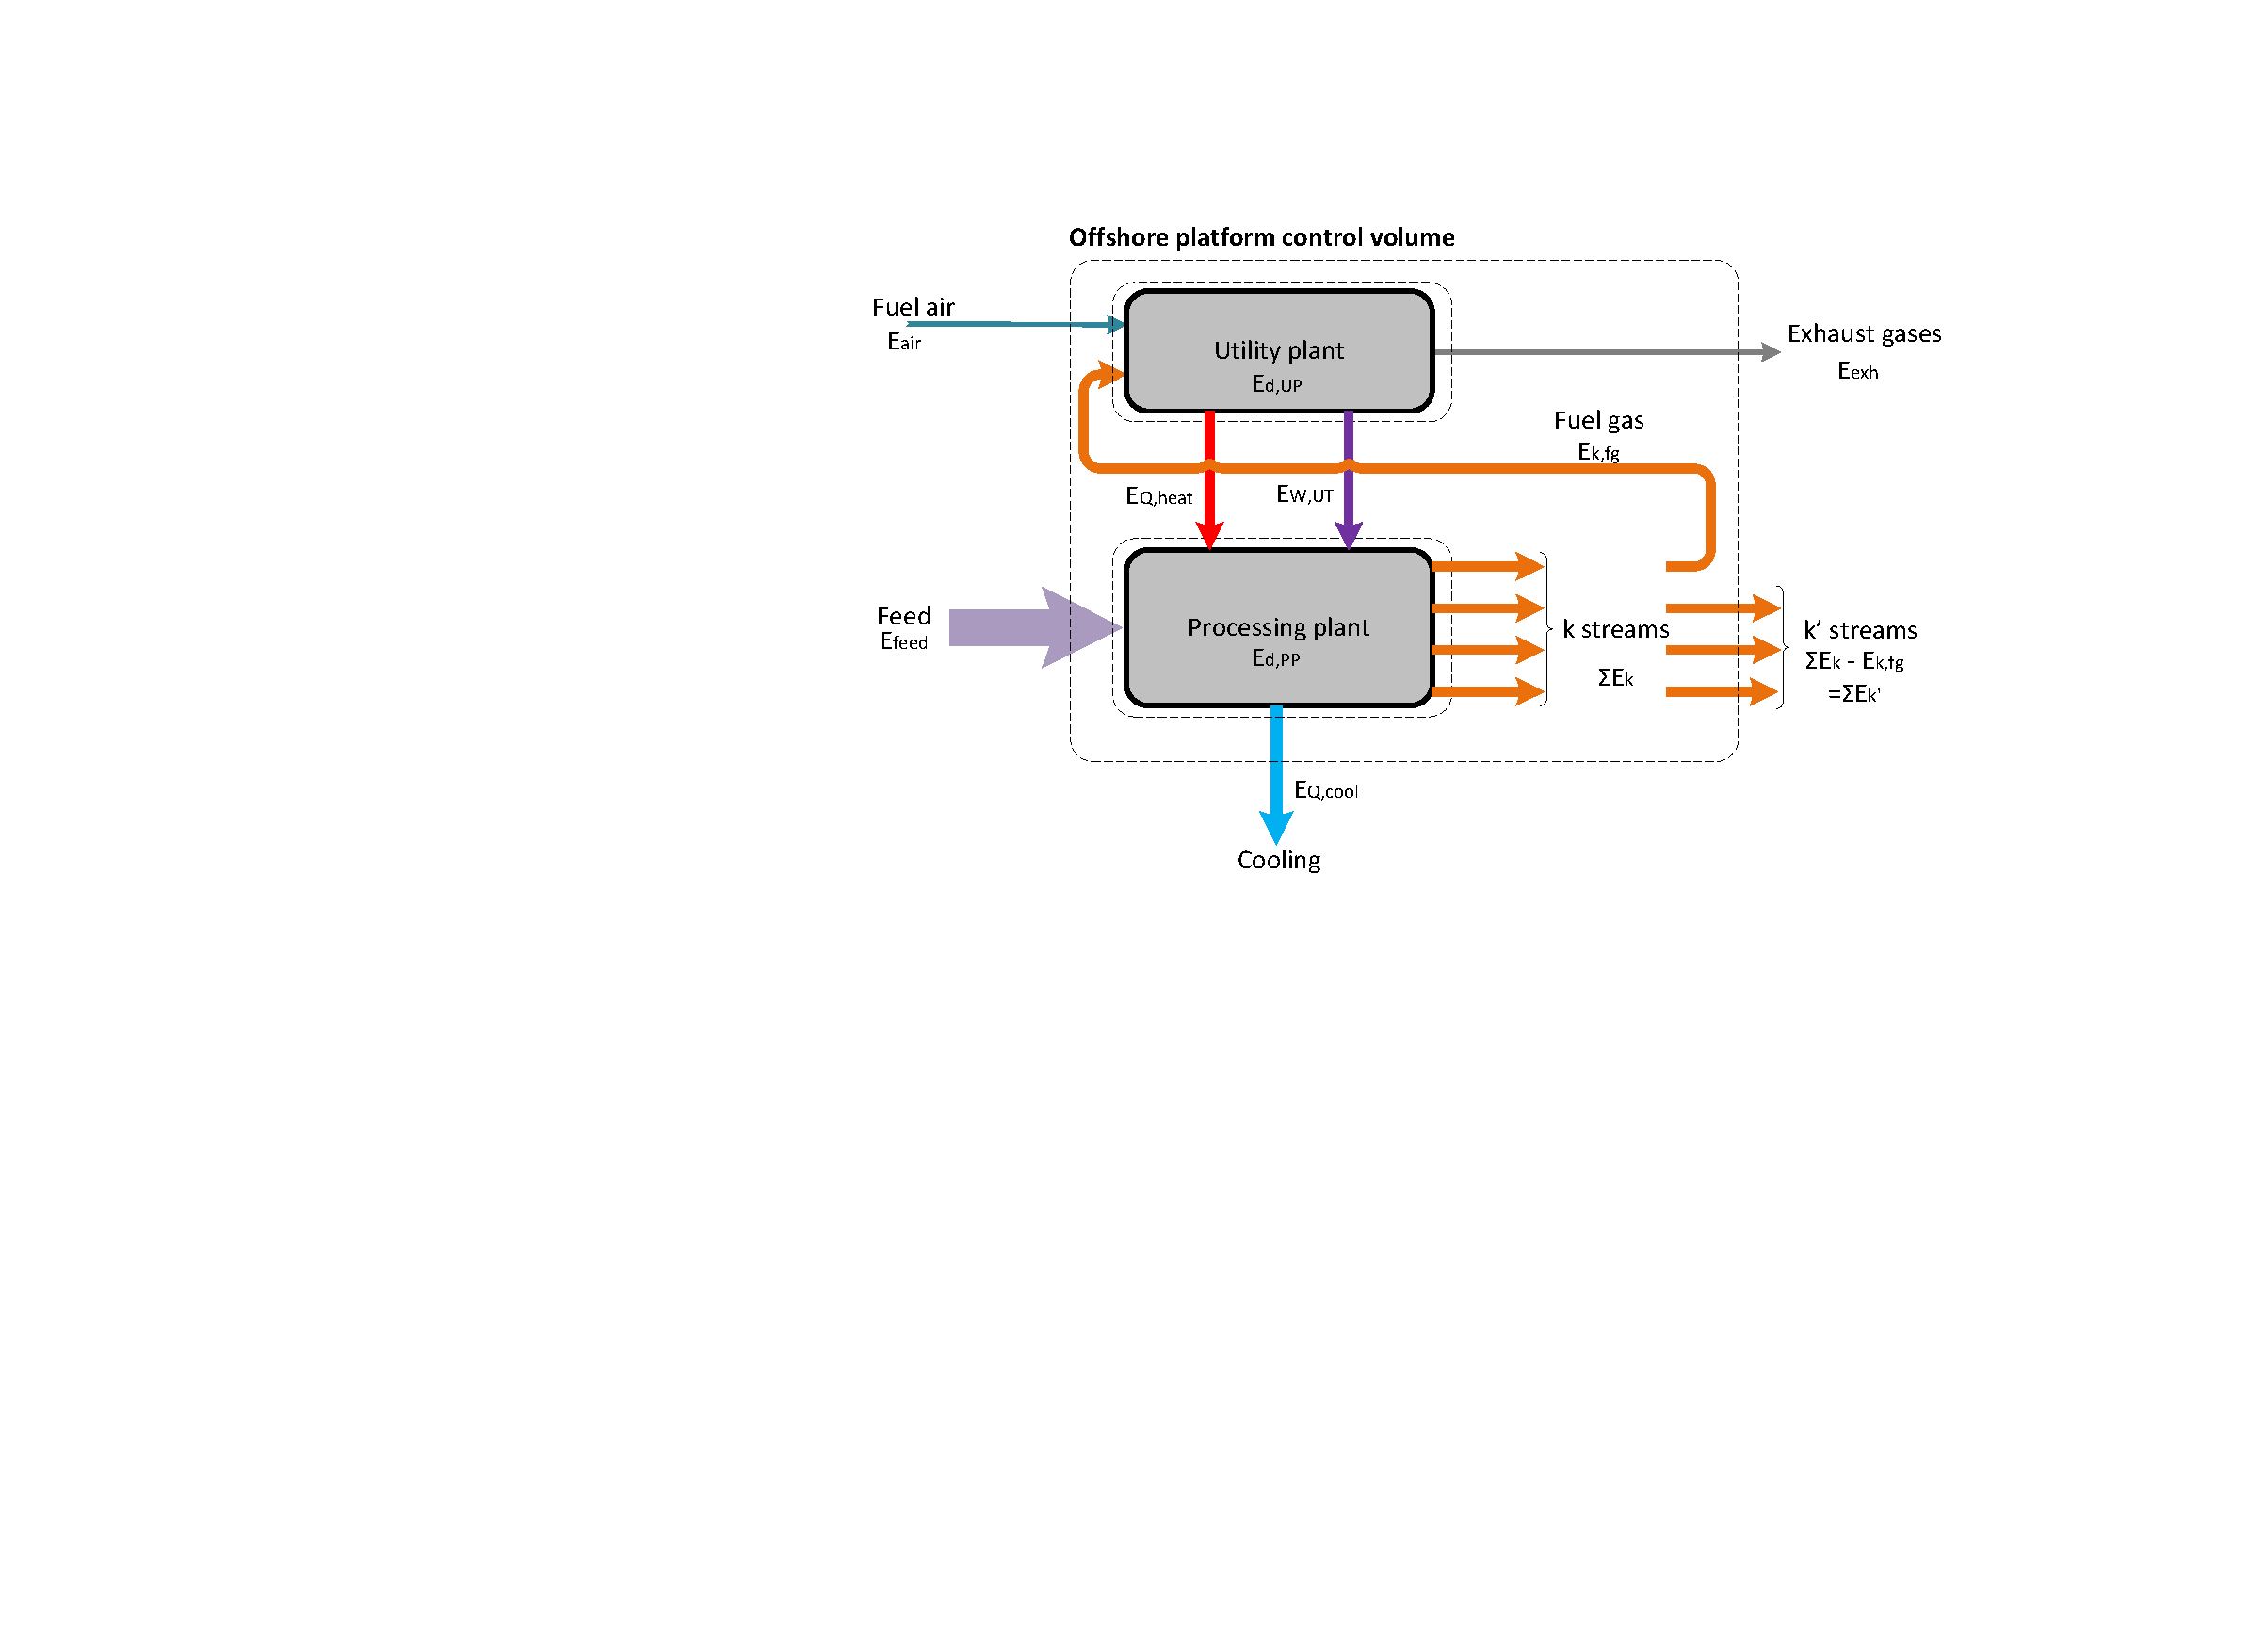
\includegraphics[width=0.75\textwidth]{control_volume.pdf}
	\caption{Control volume of oil and gas offshore facilities. \textbf{Ok to move this figure here? Maybe remove the exergy notation? But then we have to show it later again, so I don't know... What do you think, TV? Mark also that some output streams can be useful and some lost, ku and kw? Maybe best to have a very simple version here, and a version with notation in the section about efficiency?}}
	\label{fig:control_volume}
\end{figure*}

Petroleum is a complex multiphase mixture: it contains a large spectrum of chemical compounds, from light hydrocarbons in gaseous form (e.g. methane) to heavy ones in liquid phase (e.g. naphtenes and cycloalkanes) and is extracted along with subsurface water. The aim of the processing plant is to separate efficiently the different phases to satisfy the different process and export constraints, and to maximise the hydrocarbon production. Crude oil consists mostly of medium- to heavy hydrocarbons in liquid form, while natural gas mostly consists of light-weight alkanes. Differences across offshore platforms can be summarised as follows \cite{Bothamley2004,Energistyrelsen2011,NorwegianMinistryofPetroleumandEnergy2012,JonesDavidS.J.Stan;Pujado2006,Manning1991,Plisga2004,Abdel-AalH.K.;AggourMohamed;Fahim2003,VikEilanArctander;Dinning2009}: 

\begin{itemize}
	\item reservoir characteristics (e.g. initial temperature and pressure);
	\item fluid properties (e.g. chemical composition, gas- and water-to-oil (GOR and WOR)\nomenclature[A]{GOR}{Gas-to-Oil Ratio}\nomenclature[A]{WOR}{Water-to-Oil Ratio} ratios);
	\item product requirements (e.g. export pressure and temperature, chemical purity);
	\item operating strategies (e.g. oil and gas recovery, gas treatment, condensate export).
\end{itemize}
These differences induce variations in temperatures, pressures and flow rates throughout the system as well as in demands for compression, heating, cooling, dehydration, desalting and sweetening. The structural design of the processing plant stays nevertheless similar and a schematic overview is given in Figure~\ref{fig:processing_plant}.

\begin{figure*}[htbp]
	\centering
	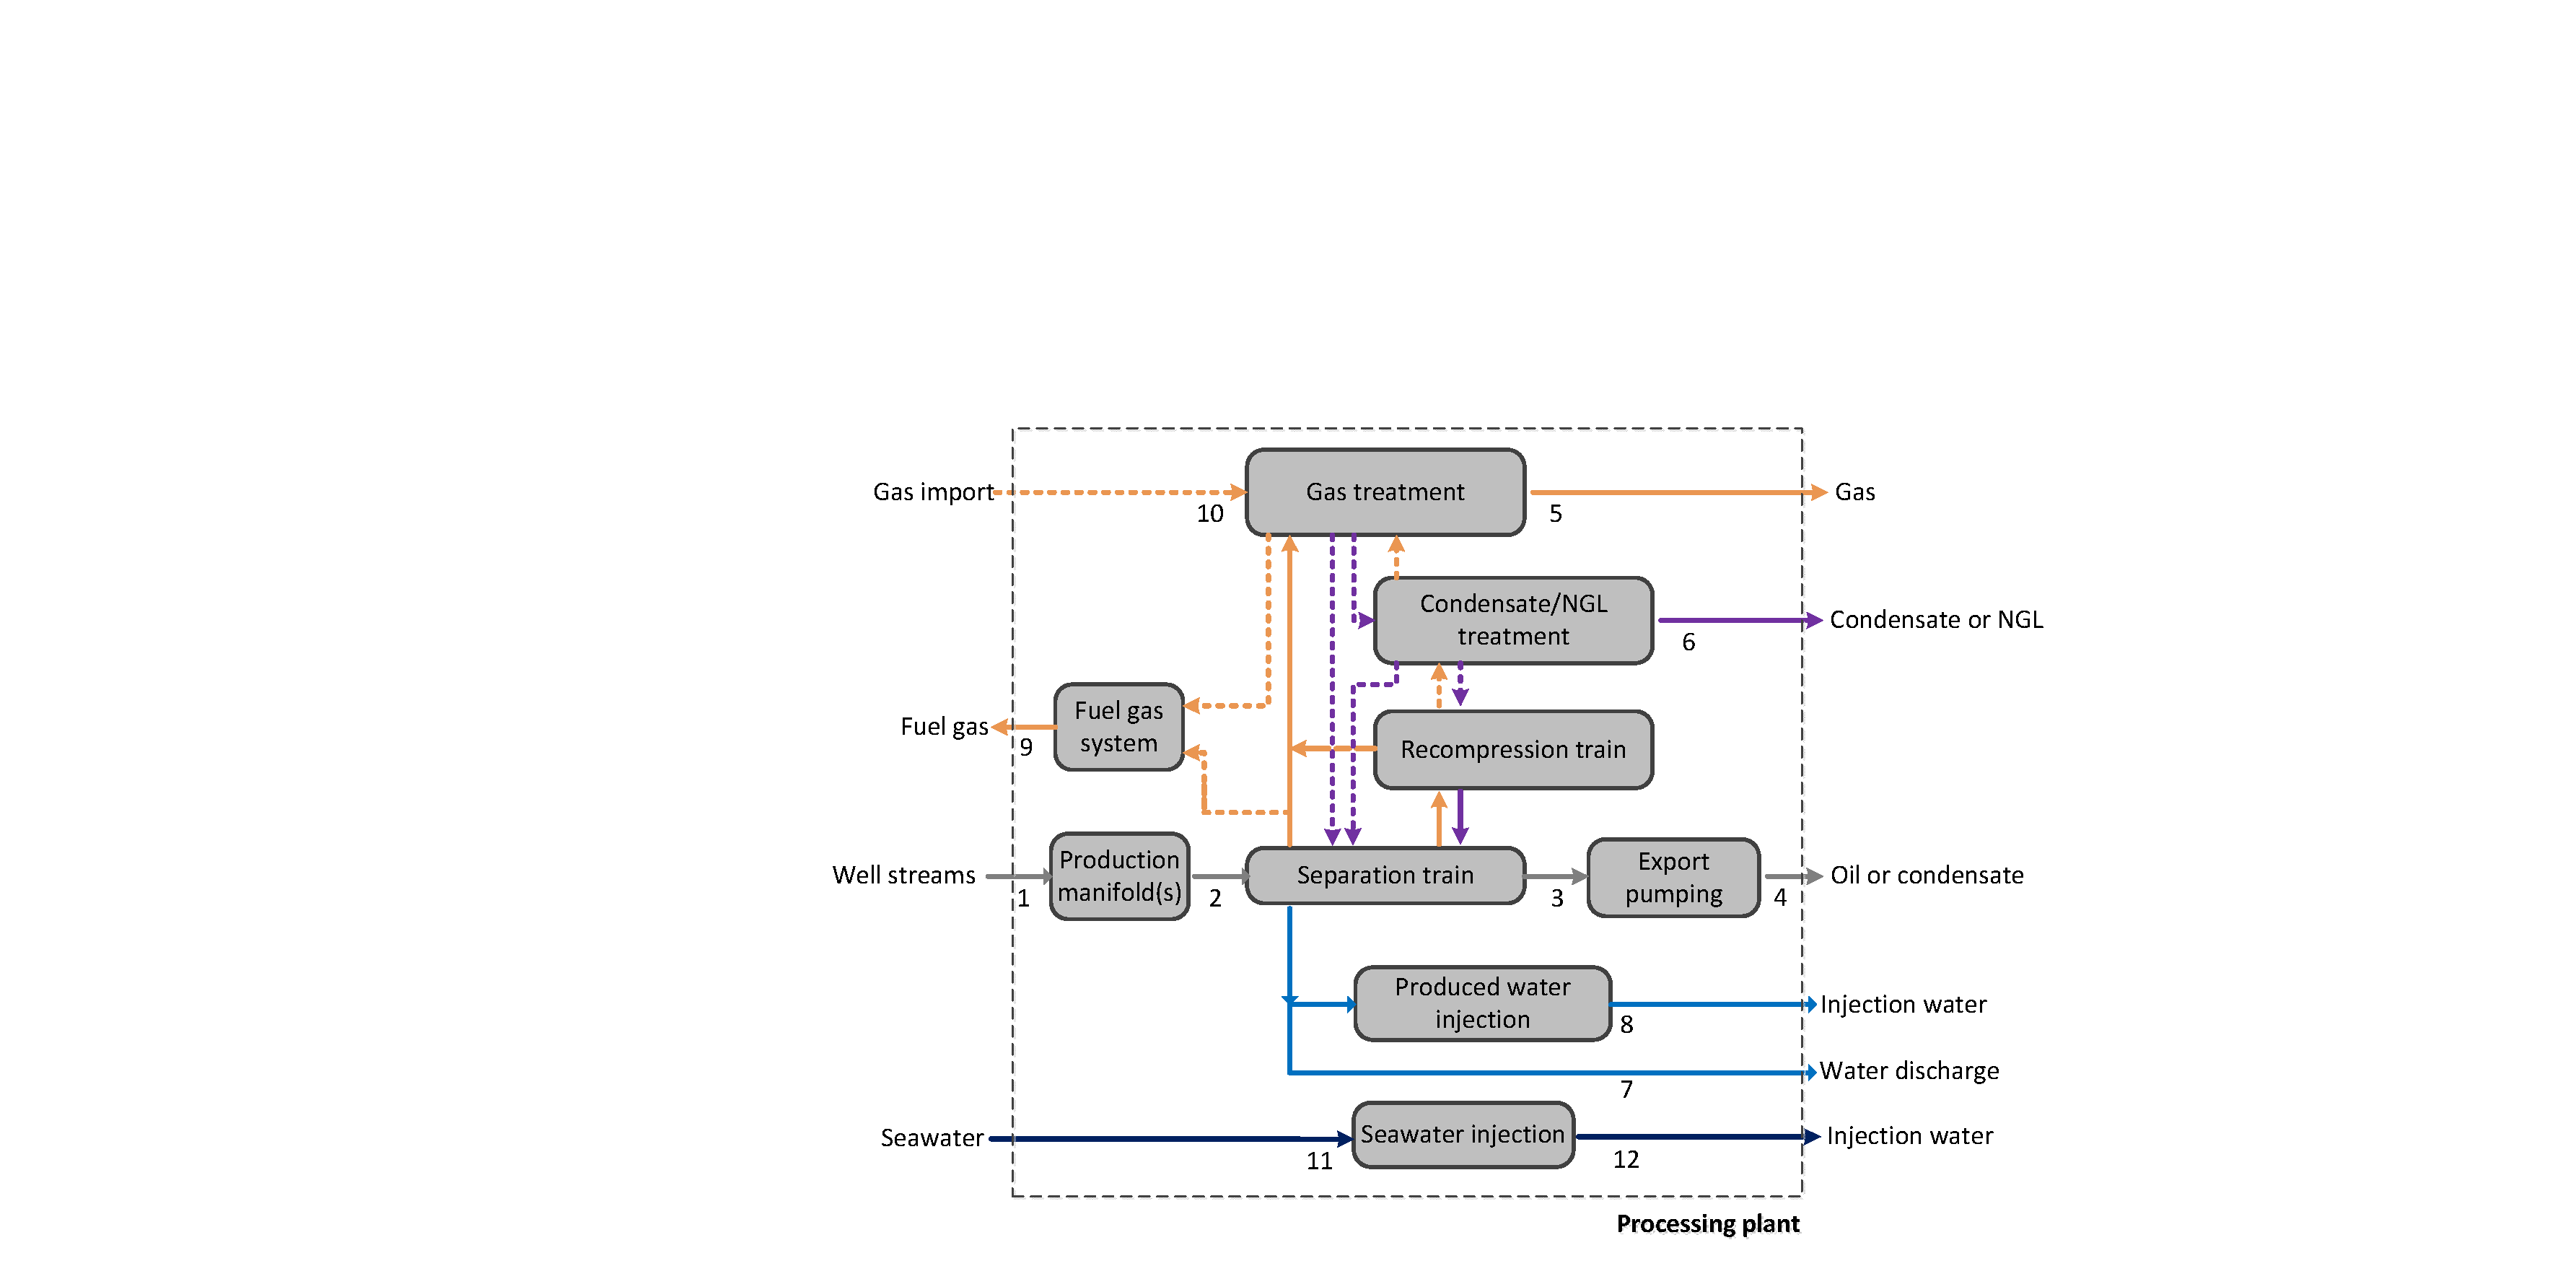
\includegraphics[width=0.75\textwidth]{general_process_overview.pdf}
	\caption{General overview of the processing plant}
	\label{fig:processing_plant}
\end{figure*}

In the processing plant oil, gas and water enter one or several production manifolds in which the well-fluid streams are mixed and the pressure reduced to ease separation between the liquid and gaseous phases. The well-fluid streams are fed into a separation system where oil, gas and water are separated by gravity in one to several stages, with throttling in between. Crude oil leaving the separation train enters a treatment and export pumping section. Gas leaving the separation and oil pumping steps enters the recompression train. It is cooled, sent to a scrubber where condensate and water droplets are removed, and recompressed to the pressure of the previous separation stage. It is then sent to the gas treatment train, where it is purified and possibly dehydrated by triethylene glycol (TEG)\nomenclature[A]{TEG}{Triethylene Glycol}. Gas may be compressed for export to the shore, lift or injection. 

Condensate removed from the recompression and gas treatment trains is (i) either sent back to the separation train and mixed with crude oil or (ii) processed apart in a condensate treatment section. Produced water enters a wastewater handling train, in which suspended particulates and dissolved hydrocarbons are removed. It is then discharged into the sea or enters an injection train where it is further cleaned and pumped to a high pressure level. In parallel, seawater may be processed onsite for further injection into the reservoir for enhanced oil recovery. 
	
The cooling demand is satisfied by using a direct cooling medium, e.g. seawater or air, or an indirect one, e.g. a glycol/water mixture. Heat exchanger networks between the several streams flowing through the system may also be integrated to promote heat integration.

Processes such as condensate treatment and natural gas liquid recovery are uncommon offshore, with only a few applications worldwide. Oil and gas treatment is generally limited to gas dehydration in the North Sea, whereas it also includes oil desalting and gas sweetening in the Gulf of Mexico. Further details on oil and gas processing are given in \cite{Manning1991a} and more specific information on North Sea platforms are given in Refs. \cite{Bothamley2004,Nguyen2013}.

\subsection{Case studies}
\label{subsec:specific}

The four oil and gas platforms investigated within this study are located in the North Sea region and present specific design characteristics (\emph{Figure \ref{fig:processing_plant}} and \emph{Table \ref{tab:platform_characteristics}}). 

\begin{table*}[htbp]
\scriptsize
  \centering
  \caption{Comparison of the four offshore facilities discussed in this study}
    \begin{tabular}{lllll}
    \toprule
    \textbf{Platform} & A     & B     & C     & D \\
    \midrule
    \textbf{System characteristics} &       &       &       &  \\
    Age (years) & 20    & 10    & 10    & 20 \\
    Gas-to-oil ratio & increasing & increasing & increasing & decreasing \\
    \textbf{} &       &       &       &  \\
    \textbf{System products} &       &       &       &  \\
    Oil   & export & none  & export & export \\
    Gas   & fuel  & fuel  & fuel  & fuel \\
          & injection & export & injection & export \\
          &       &       & import &  \\
          &       &       & lift  &  \\
    Condensate & export & export & export & export \\
          & (mixed with oil) &       & (mixed with oil) & (mixed with gas) \\
    Produced water & discharge & discharge & discharge & discharge \\
          &       &       &       & injection \\
    Seawater & cooling & cooling & cooling & cooling \\
          &       &       &       & injection \\
          &       &       &       & (complement) \\
    \textbf{Additional processes} &       &       &       &  \\
    Dehydration & n     & n     & n     & y \\
    Condensate treatment & n     & n     & n     & y \\
    Water injection  & n     & n     & n     & y \\
    \bottomrule
    \end{tabular}%
  \label{tab:platform_characteristics}%
\end{table*}%

%\begin{enumerate}
%	\item Platform A has been in operation for about 20 years and produces \emph{crude oil} and \emph{associated gas}. Crude oil is exported to another platform via pipelines for further export to the shore. Associated gas is compressed and injected into the reservoir for pressure maintenance, along with injection water produced at another platform. Produced water is treated and rejected to the sea. At the moment, oil production decreases while oil production increases.
%	\item Platform B has been in operation for about 10 years and produces \emph{gas} and \emph{condensate}. Produced gas is directly exported to the shore and recovered condensate is sent onshore via pipelines. Produced water is cleaned and discharged into a separate reservoir.
%	\item Platform C has been in operation for about 10 years and produces \emph{crude oil} and \emph{associated gas}. Gas is used for both gas lift, to ease the reservoir fluid extraction, and for gas injection, to sustain a high pressure. Produced water is also discharged into a separate reservoir. Heat integration is achieved by heat exchanges between the crude oil streams in the separation and pumping sections.
%	\item Platform D has been in operation for about 20 years and produces \emph{crude oil}, \emph{gas} and \emph{condensate}. Crude oil is stored at the bottom of the facility in oil cells and is exported onshore twice a week via shuttle tanks. Gas and condensate are dehydrated: only small amounts of gas are exported, the major fraction is used for gas lift and power generation onsite. Produced water is treated and injected back into the reservoir for pressure maintenance, alongside with seawater. Waste heat from two of the onsite gas turbines is partly recovered and used for enhancing glycol regeneration in the dehydration process and crude oil separation in the separation subsystem. 
%\end{enumerate}



These four platforms, although similar in terms of structural design, present significant differences in well-fluid processing and in operating conditions: 

\begin{itemize}
	\item The gas-to-oil ratio is either increasing (e.g. platforms A and B), meaning that the gas treatment train is run at full-design conditions or decreasing (e.g. platforms C and D), meaning that this subsystem is run in off-design conditions, and that anti-surge recycling is practiced to protect the compressors.
	\item Platforms processing heavy and viscous crude oil (e.g. platform C) or with a high propane content (e.g. platform D) require heating in the separation train to enhance vapour-liquid separation and to meet the export specifications.
	\item The pressure at the final stage of the separation train ($p_3$) is constrained by the maximum allowable vapour pressure of the crude oil/condensate in the pipelines and shuffle tankers, and is below 3 bar for all platforms.
	\item The pressure of the produced oil/condensate at the outlet of the pumping section ($p_4$) is either higher (e.g. platform C) or lower (e.g. platforms A, B and D) than at the outlet of the production manifold ($p_2$).
	\item The pressure at the outlet of the gas treatment section ($p_5$) is either higher (e.g. platforms A, C and D) or lower (e.g. platform B) than at the inlet of the separation system ($p_2$). There is a need for gas compression in three of the four platforms. 
\end{itemize} 

For more details about the processes taking place on each of these platforms, the reader is referred to two previous works conducted by the same authors \cite{Voldsund2013,Voldsund2013b}. 

\subsection{Modelling and simulation}

The process simulations were carried out with Aspen HYSYS\textsuperscript{\tiny\textregistered} \cite{Guide2004} and Aspen Plus\textsuperscript{\tiny\textregistered} version 7.2\ \cite{Technology1999}, with the exception of the glycol dehydration system. Simulations of the production manifolds, petroleum separation, oil pumping, gas recompression and flaring were based on the Peng-Robinson equation of state (EOS)\nomenclature[A]{EOS}{Equation of State} \cite{Peng1976}. The water purification and injection processes were simulated based on the Non-Random Two Liquid (NRTL) model \cite{Renon1968} and the dehydration process on the Schwartzentruber-Renon EOS \cite{Schwartzentruber1989a,Schwartzentruber1989b}. Power generation was simulated by using the in-house tool DNA (Dynamic Network Analysis), which is a program developed at the Technical University of Denmark \cite{Elmegaard2005}. 




%%%%%%%%% SECTION: THEORY %%%%%%%%%

\section{Theoretical background}
\label{sec:background}

\subsection{Exergy analysis}
\label{subsec:exergy_analysis}

\emph{Exergy} is defined as the `maximum theoretical useful work (shaft work or electrical work) as the system is brought into complete thermodynamic equilibrium with the thermodynamic environment while the system interacts with this environment only' \cite{BejanAdrian;TsatsaronisGeorge;Moran1996,Moran1998,Thermoeconomics2001}. In this work, the discussions on exergetic efficiencies focus exclusively on the exergy associated with mass and energy transfers, namely the `flow exergy'. 

Unlike energy, exergy is not conserved in real processes -- some is destroyed due to internal irreversibilities. On a time rate form and for a control volume with in- and outgoing flows, the exergy balance is expressed as: 

	\begin{align}
		\dot{E}_d&=\sum \dot{E}_{in} - \sum \dot{E}_{out} \nonumber\\
					  &=\sum \left (1-\frac{T_0}{T_k} \right ) \dot{Q}_k-\dot{W}_{cv}+\sum \dot{m}_{in} e_{in} - \sum \dot{m}_{out} e_{out}
	\end{align}

where $\dot{E}_d$, $\dot{E}_{in}$ and $\dot{E}_{out}$ are the destroyed, inflowing and outflowing exergy rates, respectively. The symbol $\dot{m}$ denotes the mass flow rate of a stream of matter, $\dot{Q}_k$ and $\dot{W}_{cv}$ the time rates of energy transfer by heat and work ($\dot{Q}\geq0$ indicates heat transfer to the system, $\dot{W}\geq0$ work done by the system) and $e$ the specific exergy of a stream of matter. The symbols $T_0$ and $T_k$ denote the environmental and instantaneous temperatures. The subscripts $in$ and $out$ denote the inlet and outlet of the system, $k$ the boundary of the component of interest and $cv$ the control volume. The exergy destruction rate can also be calculated from the Gouy-Stodola theorem, which is expressed as:

	\nomenclature[0]{$e$}{specific exergy (mass), J/kg}
	\nomenclature[S]{k}{component}
	\nomenclature[S]{cv}{control volume}
	\nomenclature[S]{in}{inlet}
	\nomenclature[S]{out}{outlet}
	\nomenclature[0]{$\dot{S}$}{Entropy rate, MW/K}
	\nomenclature[S]{gen}{generation}
	\nomenclature[0]{$p$}{pressure, MPa}
	\nomenclature[0]{$\dot{E}$}{Exergy rate, MW}
	\nomenclature[S]{d}{destruction} 
	\nomenclature[S]{l}{loss} 
	\nomenclature[S]{0}{dead state} 
	\nomenclature[P]{$^{*}$}{relative}	
	\nomenclature[0]{$T$}{Temperature, K}
	\nomenclature[P]{W}{work} 
	\nomenclature[P]{Q}{heat} 
	
	\begin{equation}
		\dot{E}_d=T_0\dot{S}_{gen}
	\end{equation}
	
	where $\dot{S}_{gen}$ is the entropy generation rate.

Exergy destruction is also called `internal exergy losses', since this is exergy that is lost related to the irreversibilities taking place \emph{inside} the control volume under study. The term exergy loss, written $\dot{E}_l$ \cite{BejanAdrian;TsatsaronisGeorge;Moran1996} refers to the exergy discharged to the environment without any practical use (e.g. exergy content of exhaust gases from a gas turbine -- exergy transferred to the cooling water), i.e. \emph{outside} the control volume under study. This waste exergy is destroyed when mixed irreversibly with the environment (\emph{Figure \ref{fig:balance}}) and is denoted `external exergy losses' in the works of Szargut and Kotas \cite{Szargut1998,Kotas1995}. 

Kostenko \cite{Kostenko1983} and later Brodyansky \cite{Brodyansky1994} introduced the concept of \emph{`transit exergy'} $\dot{E}_{tr}$, which is the part of the exergy supplied to a system that flows through the system without undergoing any physical or chemical transformation. By opposition, they named the fraction of the exergy flowing into the system that is not transit exergy \emph{`consumed exergy'} and the fraction of the exergy flowing out that is not transit exergy\emph{`produced exergy'}. Transit exergy can be divided into the transit exergy carried with the waste streams $\dot{E}_{tr,l}$ and carried with the utilisable streams $\dot{E}_{tr,u}$. 


\textbf{Introduce the exergy balance.}
Hence, the exergetic balance becomes \cite{BejanAdrian;TsatsaronisGeorge;Moran1996,Tsatsaronis2007}:

\begin{equation}
\dot{E}_p=\dot{E}_f-\dot{E}_l-\dot{E}_d
\end{equation}
\nomenclature[S]{p}{product}
\nomenclature[S]{f}{fuel}
\nomenclature[G]{$\varepsilon$}{exergetic efficiency}
		
The general concept of `fuel' and `product' has been extensively applied over the last decades to characterise the thermodynamic performance of various systems \cite{Tsatsaronis1985,Thermoeconomics2001,BejanAdrian;TsatsaronisGeorge;Moran1996,Tsatsaronis1993}. 

\begin{figure*}[htbp]
	\centering
	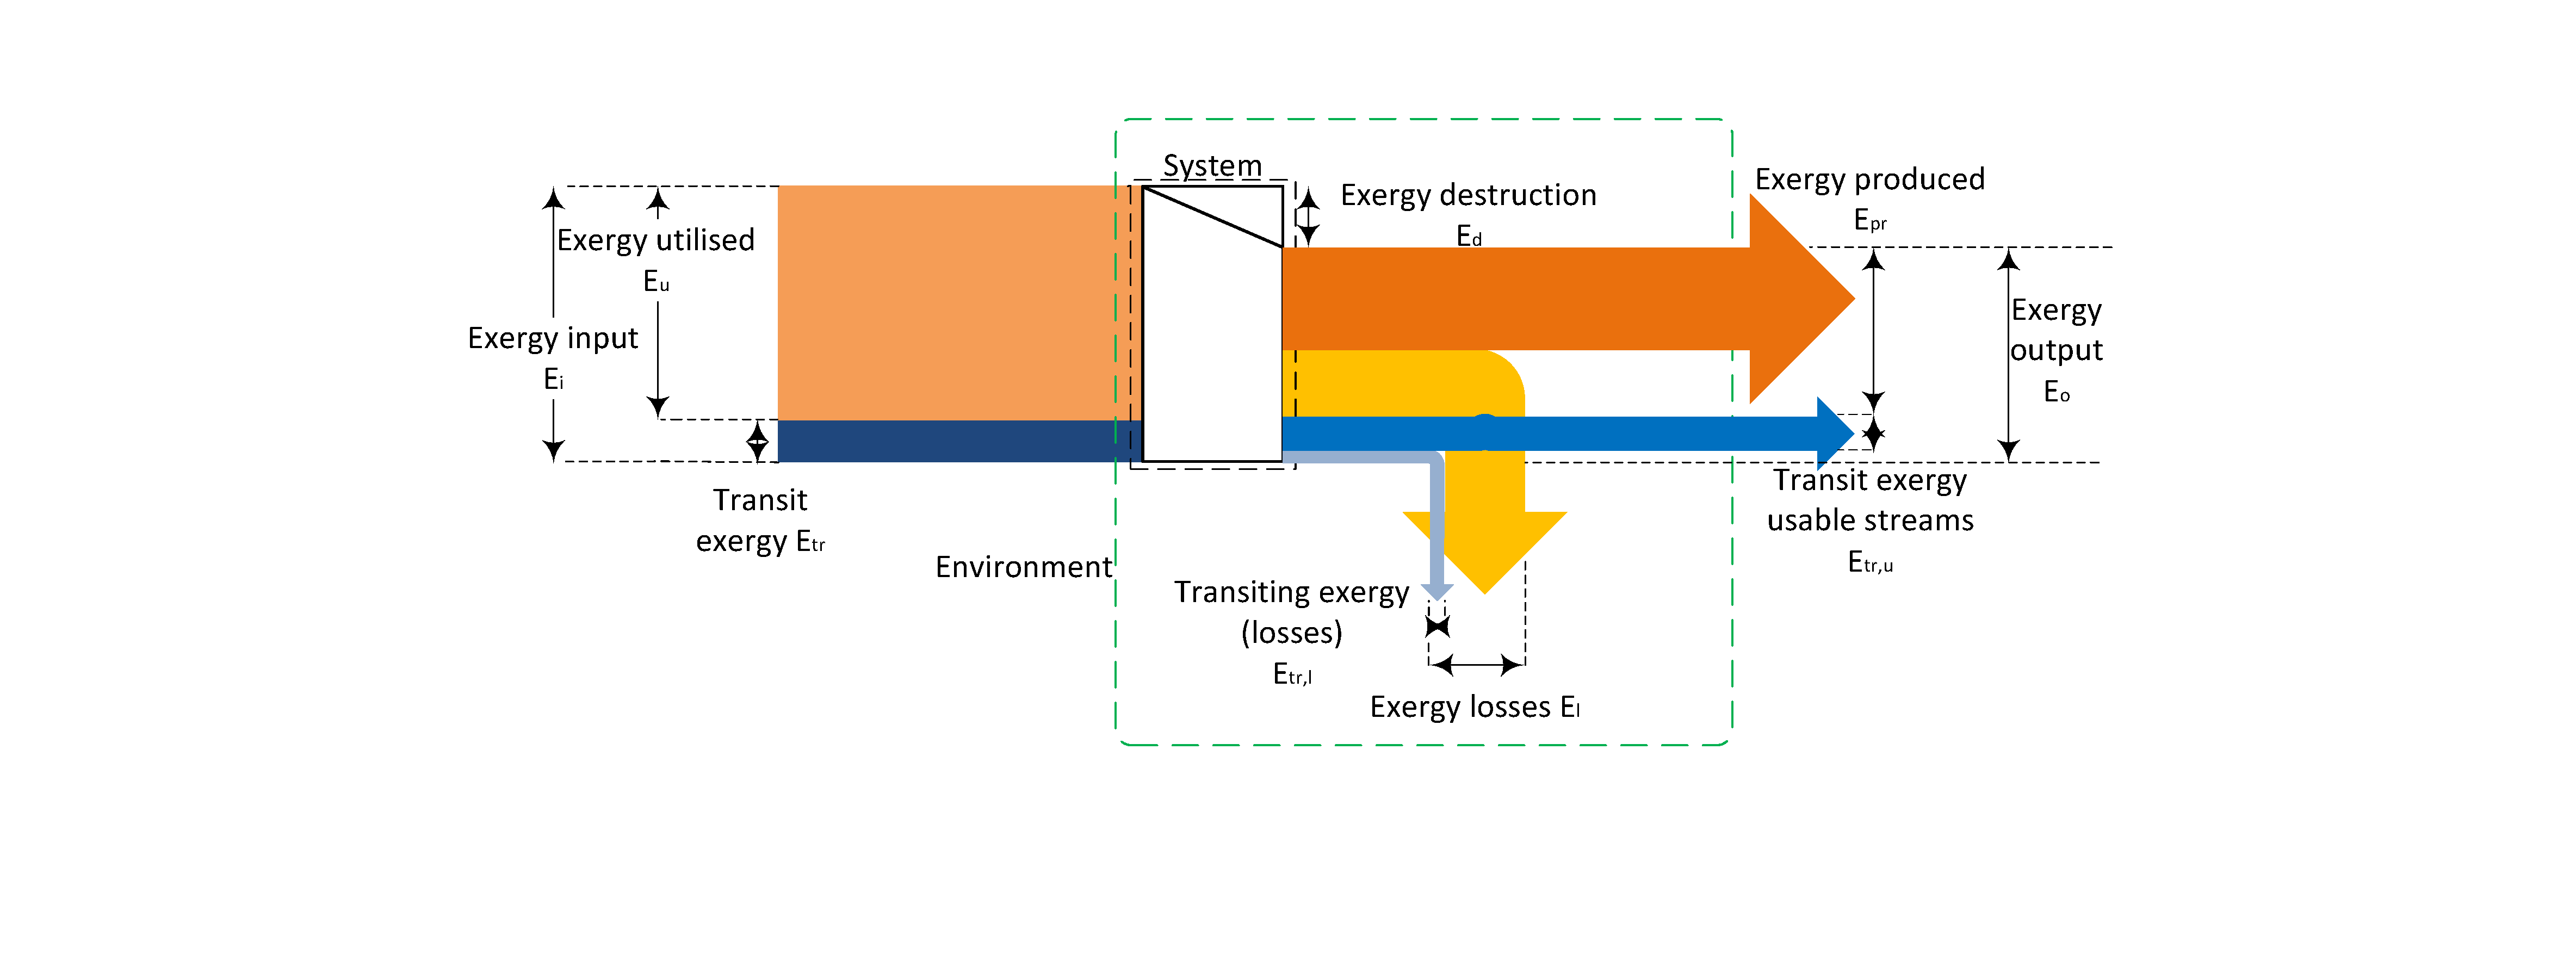
\includegraphics[width=\linewidth]{balance.pdf}
	\caption{Conceptual representation of the exergy balance}
	\label{fig:balance}
\end{figure*}
	
\subsection{Flow exergy}

In the absence of nuclear, magnetic and electrical interactions, the exergy associated with a stream of matter is a function of its physical $e^{ph}$, chemical $e^{ch}$, kinetic $e^{kin}$ and potential $e^{pot}$ components \cite{BejanAdrian;TsatsaronisGeorge;Moran1996}. The specific exergy of a material stream, on a mass basis, is expressed as:

	\nomenclature[P]{ph}{physical} 
	\nomenclature[P]{ch}{chemical} 
	\nomenclature[P]{kin}{kinetic} 
	\nomenclature[P]{pot}{potential} 
	\nomenclature[0]{$\bar{e}$}{specific exergy (molar), J/mol} 
	\nomenclature[0]{$y$}{component/sub-system exergy ratio} 
		
	\begin{equation}
		e=e^{ph}+e^{ch}+e^{kin}+e^{pot}
	\end{equation}

Physical exergy accounts for temperature and pressure differences from the environmental state and is defined as:  
		
	\begin{equation}
		e^{ph}=(h-h_0)-T_0(s-s_0)=\underbrace{h-h(T_0,p)-T_0\left(s-s(T_0,p)\right)}_{I}+\underbrace{h-h(T,p_0)-T_0\left(s-s(T,p_0)\right)}_{II}
	\end{equation}
	
	where $h$ and $s$ are the specific enthalpy and entropy of a stream of matter per unit-of-mass, respectively. \emph{Term I} and \emph{Term II} refer to the the temperature- and pressure-based components of the physical exergy \cite{Kotas1995}, respectively, and are also named thermal $e^{t}$ and mechanical $e^{m}$ exergies \cite{Tsatsaronis1993}.

\nomenclature[P]{t}{thermal} 
\nomenclature[P]{m}{mechanical} 

Chemical exergy accounts for deviations in chemical composition from reference substances present in the environment. In this work, chemical exergy is calculated using the reference environment defined in Szargut \cite{Szargut1988,Szargut1989,Morris1986}. The specific chemical exergy of a given mixture $\bar{e}^{ch}_{mix}$, on a molar basis, is expressed as \cite{Sato2004}:

\begin{equation*}
	\bar{e}^{ch}_{mix}=\underbrace{\sum_i \bar{x}_i \bar{e}^{ch}_{i,mix}}_{I}=\underbrace{\sum_i \bar{x}_i \bar{e}^{ch}_{i,0}}_{II}+\underbrace{\left(\sum_i \bar{x}_i \left(h_{i,mix}-h_{i,0}\right)\right)-T_0\left(\sum_i \bar{x}_i \left(s_{i,mix}-s_{i,0}\right)\right)}_{III}
\end{equation*}

	where the molar fraction, the chemical compound and the mixture are denoted by $\bar{x}$, $i$ and $mix$, respectively. The specific molar exergy of a given chemical compound is written $\bar{e}^{ch}_{i,mix}$ when it is in the mixture and $\bar{e}^{ch}_{i,0}$ when it is in a pure component state. The term $I$ illustrates the chemical exergy of each individual chemical component in the mixture, the term $II$ the chemical exergy of these components in an unmixed form and the term $III$ the reduction in chemical exergy due to mixing effects.  

\nomenclature[S]{i}{chemical compound}
\nomenclature[S]{mix}{mixture}

If no chemical transformations are taking place within a separation system, the terms related to the chemical exergy of pure components cancel and the change in chemical exergy is equal to the exergy used to perform the separation work \cite{Kotas1995}. The variation of chemical exergy between the inlet and the outlet of that system, which is, in this specific case, equal to the exergy used for separation, can be expressed as:

\begin{equation}
\Delta \dot{E}^{ch} = \sum_k \dot{E}^{ch}_k-\dot{E}^{ch}_{mix} = \sum_k \left( \sum_i \dot{n}_{i,k} \left(h_{i,k}-h_{i,mix}\right)-T_0\left(\sum_i \dot{n}_{i,k}\left(s_{i,k}-s_{i,mix}\right)\right)\right) = \sum_k \Delta \dot{E}^{ch}_k
\end{equation}

	where $\Delta \dot{E}^{ch}_k$ corresponds to the exergy used for separation into each stream $k$ exiting the system:

\begin{equation}
\Delta \dot{E}^{ch}_k = \left(\sum_i \dot{n}_{i,k} \left(h_{i,k}-h_{i,mix}\right)\right)-T_0\left(\sum_i \dot{n}_{i,k}\left(s_{i,k}-s_{i,mix}\right)\right)
\end{equation}	

The specific chemical exergy of hypothetical components $\bar{e}^{ch}_h$ is determined with the heuristic correlations of Rivero \cite{Rivero1999}:
	
\begin{equation}
	\bar{e}^{ch}_h=\beta NHV_h+\sum \bar{z}_{mt} \bar{e}^{ch}_{mt}
\end{equation}
	
	\nomenclature[0]{$z$}{pollutant molar fraction}
	\nomenclature[0]{$h$}{specific enthalpy (mass), J/kg}
	\nomenclature[0]{$s$}{specific entropy (mass), J/(kg$\cdot$K)}
	\nomenclature[S]{h}{hypothetical}
	\nomenclature[S]{mt}{metal}
	\nomenclature[A]{NHV}{Net Heating Value, kJ/kmol}
	
	where $NHV$ stands for Net Heating Value, $z_{mt}$ for the mass fraction of metal impurities, $e^{ch}_{mt}$ for the corresponding chemical exergy and $\beta$ for the chemical exergy correction factor.

	\nomenclature[G]{$\beta$}{chemical exergy correction factor}
	
Kinetic and potential contributions on the flow exergies were assumed to be negligible toward physical and chemical exergies. Exergy transported with work is equal to its energy and depends on the system and environmental temperatures when it is transferred with heat.

\subsubsection{Transit exergy}

The transiting exergy associated with a stream of matter is defined as the sum of the transiting physical, chemical, potential and kinetic exergies. The transiting physical exergy for a stream $j$ is the minimum physical exergy between the inlet and outlet of the system. It is defined, for an input and output temperature higher than the environment temperature, as:

\begin{equation}
\dot{E}^{ph}_{tr} = \sum_j \dot{m}_{j,tr}\cdot\text{min}(e^{ph}_{in}(p_{in},T_{min});e_{in}^{ph}(p_{out},T_{min});e_{o}^{ph}(p_{in},T_{min});e_{out}^{ph}(p_{out},T_{min}))
\end{equation}
\nomenclature[S]{min}{minimum} 

Similarly, the transiting chemical exergy corresponds to the chemical exergies of each chemical compound that is not transformed between the system inlet and outlet:

\begin{equation}
\dot{E}^{ch}_{tr} = \sum_s \dot{n}_{tr,s}\cdot\text{min}(\bar{e}^{ch}_i,\bar{e}^{ch}_o)
\end{equation}
\nomenclature[S]{j}{stream}

The transiting exergies of an energy flow are defined as the minimum associated exergies at the inlet or outlet of the system. The concept of transiting exergy is also mentioned by Cornelissen \cite{Cornelissen1997}, who applied this method to an air separation unit and a crude oil distillation plant. The lack of ambiguity and the complexity of the calculations were underlined, as this method requires a precise decoupling of the exergy flows into their components.
	
%%%%%%%%% SECTION: THEORY: EXERGETIC EFFICIENCY %%%%%%%%%%%%%%%%%%%%%%%%%%%%%%%%%%%%%%%%%%%%%%%%%%%%%%%%%%%%%%%%%%%%%%%%%%%%%%%%%%%%%%%

\subsection{Exergetic efficiency}

The definitions of exergetic efficiency, as presented and discussed in the open literature, can be divided into two main groups, as suggested by Lior and Zhang \cite{Lior2007}:

\begin{itemize}
	\item the \emph{`total'}, \emph{`overall'}, \emph{`input-output'} or \emph{`universal'} exergetic efficiency, which is defined as the ratio of all outgoing to ingoing exergy flows, without any consideration on whether they are actually consumed within the process or useful to the owner of the system;
	\item the \emph{`task'}, \emph{`utilitarian'}, \emph{`consumed-produced'}, or \emph{`functional'} \textbf{(rational?)} exergetic efficiency, which is defined as the ratio of the exergy terms associated with the products generated within the system, i.e. the \emph{`produced exergy'}, to the exergy terms associated with the resources expended to achieve these outputs, i.e. the \emph{`consumed exergy'}.
\end{itemize}

\subsubsection{Total exergetic efficiency}

For a given open thermodynamic system at steady-state, the exergy balance can be expressed as:
\begin{equation}
	\sum \dot{E}_{in} = \sum \dot{E}_{out}+\dot{E}_d = \sum \dot{E}_{out,u} + \sum \dot{E}_{out,l} + \dot{E}_d
\end{equation}
where $\dot{E}_{in}$ and $\dot{E}_{out}$ are the exergy inputs and outputs to and from the system, associated with streams of matter and of energy, and $\dot{E}_d$ the exergy destruction. The exergy output consists of useful exergy output, $\dot{E}_{out,u}$, and exergy that is lost (i.e. the exergy of waste products that is not taken into use, but discharged to the environment), $\dot{E}_{out,l}$.

The \emph{`total'} exergetic efficiency $\varepsilon_t$ is defined as the ratio of all exergy outflows to inflows \cite{Cornelissen1997,Lior2007,Wall2004}:
\begin{equation}
	\varepsilon_t \equiv \frac{\sum \dot{E}_{out}}{\sum \dot{E}_{in}} = 1-\frac{\dot{E}_d}{\sum \dot{E}_{in}}
\end{equation}
where some authors exclude the exergy associated with waste products \cite{Fratzscher1986,Wall2004}:
\begin{equation}
	\varepsilon_t \equiv \frac{\sum \dot{E}_{out,u}}{\sum \dot{E}_{in}} = 1-\frac{\dot{E}_{out,l}+\dot{E}_d}{\sum \dot{E}_{in}}
\end{equation} 

The \emph{'total'} exergetic efficiency is claimed to be adequate when (i) the ingoing and outgoing exergy flows are converted to other forms of exergy \cite{Cornelissen1997} or (ii) a major part of the outflowing exergy can be considered as useful, as it is the case of power plants \cite{Lior2007} or (iii) for dissipative processes and devices \cite{Moran1989,Kotas1995}. 

 
\subsubsection{Task exergetic efficiency}

The concept of \emph{`total'} exergetic efficiency has been criticised as it takes into account all the exergetic flows entering and exiting a system, without considering whether they are utilised in the thermodynamic conversions. The \emph{`task'} exergetic efficiency, on the opposite, differentiates the exergy flows undergoing transformations from the exergy flows that are not affected, i.e. neither used nor produced. Grassmann \cite{Grassmann1950} proposed a general formulation for an exergetic efficiency: he suggested the ratio of the intended increase to the used decrease in ability to do work. In exergy terms, this means that the exergetic efficiency should be defined as the ratio of the production of exergy that is desired $\Delta \dot{E}^+$ to the reduction of exergy that is utilised $\Delta \dot{E}^-$.

\begin{equation}
	\varepsilon \equiv \frac{\Delta \dot{E}^+}{\Delta \dot{E}^-}
\end{equation}

It was emphasised that this performance criterion always has a value comprised between 0 and 1, as the increased ability to do work $\Delta \dot{E}^+$ is always smaller than the decreased one $\Delta \dot{E}^-$. Baehr \cite{Baehr1968} proposed a variant of this formulation, considering \emph{all} the exergy increases $\Delta \dot{E}^+_t$ in the numerator and \emph{all} the exergy decreases $\Delta \dot{E}^-_t$ in the denominator. At the difference of the expression proposed by Grassmann \cite{Grassmann1950}, the total production and expenditure of exergy are considered, whether they are actually desired or utilised within the system:

\begin{equation}
	\varepsilon \equiv \frac{\Delta \dot{E}^+_{tot}}{\Delta \dot{E}^-_{tot}}
\end{equation}

\nomenclature[P]{+}{increase}
\nomenclature[P]{-}{decrease} 
\nomenclature[S]{tot}{total} 
\nomenclature[S]{cv}{control volume} 
It was pointed up that (i) exergetic efficiencies based on exergy differences are more sensitive to changes in the system and are therefore more suitable and (ii) different numerical values could be obtained with the formulation of exergetic efficiency proposed by Grassmann \cite{Grassmann1950}, as it depends on whether an exergy difference is considered as \emph{`useful'}, \emph{`used'} or none of those.

\nomenclature[S]{tr}{transit}

Brodyansky \cite{Brodyansky1994} and Sorin \cite{Sorin1994} proposed to define the exergetic efficiency as the ratio of the total exergy output to the total exergy input, minus the transit exergy on both numerator and denominator. They named it the \emph{intrinsic exergetic efficiency} and defined it as:

\begin{equation}
\varepsilon \equiv \frac{\sum \dot{E}_{out}-\sum \dot{E}_{tr}}{\sum \dot{E}_{in}-\sum \dot{E}_{tr}} = \frac{\sum \dot{E}_{pr}}{\sum \dot{E}_u}
\end{equation}

	where, on a time rate basis, $\dot{E}_{tr}$ the transit exergy, $\dot{E}_{pr}$ and $\dot{E}_{u}$ the produced and used exergies, respectively, as called in the work of Brodyansky et al. \cite{Brodyansky1994}.  

A variant of the previous exergy efficiency formulation is proposed by Sorin et al. \cite{Sorin1998}. It was argued that all the produced exergy $\dot{E}_{pr}$ it not usable, as a result of a discharge of exergy into the environment with waste products (i.e. external exergy losses). They defined therefore an alternative to the intrinsic exergetic efficiency, named the utilisable exergy coefficient, as:

\begin{equation}
\varepsilon \equiv \frac{\sum \dot{E}_{o}-\sum \dot{E}_{l}-\sum \dot{E}_{tr,u}}{\sum \dot{E}_{i}-\sum \dot{E}_{tr,u}}
\end{equation}

 Szargut \cite{Szargut1980,Szargut1988,Szargut1998}, Tsatsaronis \cite{Tsatsaronis1985} and Kotas \cite{Kotas1980a,Kotas1995} argued that the exergetic efficiency should be defined as the ratio of (i) the \emph{desired output} or \emph{useful exergetic effect} $\sum \Delta \dot{E}_{out}$ and (ii) the \emph{necessary input} or \emph{driving exergy expense} $\sum \Delta \dot{E}_{in}$. Both terms can be identified starting from the exergy balance put in the following form:

\begin{equation}
	\sum \Delta \dot{E}_{in}=\sum \Delta \dot{E}_{out}+\dot{I}_{cv}
\end{equation} 
 
	where $\dot{I}_{cv}$ is defined as the irreversibilities taking place within the control volume under consideration, on a rate form. Hence, the proposed efficiency, named `rational' efficiency, is defined, for any system for which a useful output can be expressed in terms of exergy \cite{Kotas1980a,BejanAdrian;TsatsaronisGeorge;Moran1996}, as: 
 
 \begin{equation}
	\varepsilon \equiv \frac{\sum \Delta \dot{E}_{out}}{\sum \Delta \dot{E}_{in}}
\end{equation}
 
Using the nomenclature proposed by Tsatsaronis \cite{Tsatsaronis2007}, the rational exergetic efficiency, or simply called the \emph{`exergy efficiency'} in the works of Moran \cite{Moran1989,Moran2007}, Lazzaretto \cite{Lazzaretto1999,Lazzaretto2006} and Valero \cite{Valero1987} can be written as:

\begin{equation}
	\varepsilon \equiv \frac{\dot{E}_p}{\dot{E}_f} = 1-\frac{\dot{E}_l+\dot{E}_d}{\dot{E}_f}
\end{equation} 

%%%%%%%%% SECTION: EFFICIENCIES FOR OIL AND GAS PLATFORMS %%%%%%%%%%%%%%%%%%%%%%%%%%%%%%%%%%%%%%%%%%%%%%%%%%%%%%%%%%%%%%%%%%%%%%%%%%%%%%%%%%
 
 \section{Exergetic efficiency for oil and gas platforms}
 \label{sec:efficiency}
 
As described in \emph{Section~\ref{sec:system_description}}, we use three different control volumes when analysing an oil platform; the utility plant, the processing plant and the overall plant. In this section we establish the exergy balance for each of these control volumes and derive expressions for exergetic efficiency. For the utility plant the \emph{`total'} exergetic efficiency is suitable, but for the processing plant and overall plant, the formulation of exergetic efficiency is not straightforward. This is due to (i) high transit chemical (and sometimes also physical) exergy and (ii) high variety in process conditions and product specifications among the platforms. \textbf{(more?)} For these two control volumes we have found several different expressions for the exergetic efficiencies for similar systems in the literature \cite{Oliveira1997,Cornelissen1997,Voldsund2010,Voldsund2012,Voldsund2013,Rian2012,Thermoeconomics2001}. 

\textbf{For both the \emph{`total'} exergetic efficiency and the \emph{`task'} exergetic efficiency some authors have included all product or all output flows, while others have only considered the \emph{useful} products or output flows. Note that in this work we will only consider \emph{useful} products or output flows.}


%For oil and gas systems where material streams exiting the processing plant are discharged into the environment without any practical use (e.g. produced water, flared and vented gases), the exergy losses are identified as the sum of the exergy discharged to the sea via cooling, the exergy contents of the exhaust gases \emph{and} of the waste streams of the processing plant. \textbf{Merge into the paragraph above.} In some works these streams are also regarded as product streams, while in this work we do not regard these streams as product. 


%Due to high transit chemical exergy, the 'input-output' exergetic efficiency will give a number close to 1, that do not give much useful information. 

%Only the formulations of the exergetic efficiencies based on the fuel-product concept are discussed, as the input-output and intrinsic efficiencies are calculated in a systematic way, using the algorithms presented in \emph{Section \ref{sec:background}} \textbf{Direct result of the exergy balances presented in Section~\ref{section:exergy_balances}.}


%%%%%%%%%%%%%%%%%%%%%%%%%%%%%%%%%%%%%%%%%%%%%%%%%%%%%%%%%%%%%%%%%%%%%%%%%%%%%%%%%%%%%%%%%%%%%%%%%%
 
%\subsection{Exergy balances}
%\label{section:exergy_balances}
 
%The exergy balance for the processing plant of the oil and gas facility (\emph{Figure \ref{fig:control_volume}}) can be expressed as:

%\begin{equation}
%	\dot{E}_{feed}+\dot{E}^{Q}_{heat}+\dot{E}^{W}_{UT}=\sum_k\dot{E}_k+\dot{E}^{Q}_{cool}+\dot{E}_{d,PP}
%\end{equation}

%The left-hand side (LHS) term represents, on a time rate basis, the exergy associated with the feed entering the processing plant (i.e. reservoir fluid) $\dot{E}_{feed}$ and the exergy transfers with the heating medium $\dot{E}^{Q}_{heat}$ and power $\dot{E}^{W}_{UT}$ from the utility plant that are consumed within the separation and treatment modules. The right-hand side (RHS) term denotes the exergy of the outlet streams of the processing plant (i.e. oil, gas, condensate, flared gas, fuel gas, produced water) $\sum_k\dot{E}_k$ and the exergy gain discarded with the cooling medium discharged to the environment $\dot{E}^{Q}_{cool}$. $\dot{E}_{d,PP}$ is the exergy destroyed in the processing plant. 

%\nomenclature[S]{cool}{cooling medium}
%\nomenclature[S]{feed}{feed}
%\nomenclature[A]{UT}{Utility Plant}
%\nomenclature[A]{PP}{Processing Plant}
%\nomenclature[A]{OP}{Overall Plant}
%\nomenclature[A]{LHS}{Left-Hand Side}
%\nomenclature[A]{RHS}{Right-Hand Side}	
	
%The exergy balance for the utility plant of the oil and gas facility (\emph{Figure \ref{fig:control_volume}}) can be expressed as:
	
%\begin{equation}
%	\dot{E}_{air}+\dot{E}_{k,fg}=\dot{E}^{Q}_{heat}+\dot{E}^{W}_{UT}+\dot{E}_{exh}+\dot{E}_{d,UT}
%\end{equation}

%The left-hand side (LHS) term represents, on a time rate basis, the exergy entering the utility plant that are associated with the air $\dot{E}_{air}$ and fuel gas $\dot{E}_{k,fg}$ from the separation plant. The right-hand side (RHS) term denotes the exergy accompanying the power $\dot{E}^{W}_{UT}$ and heat $\dot{E}^{Q}_{heat}$ produced in the utility plant and $\dot{E}_{exh}$ the exergy rejected into the environment with the exhaust gases. $\dot{E}_{d,UT}$ is the exergy destroyed in the utility plant.

%Hence, for the overall plant, i.e. the combination of the processing and utility plants (\emph{Figure \ref{fig:control_volume}}), the exergy balance becomes:

%\begin{align}
%	\dot{E}_{feed}+\dot{E}_{air}&=\left(\sum_k\dot{E}_k-\dot{E}_{k,fg}\right)+\dot{E}^{Q}_{cool}+\dot{E}_{exh}+\dot{E}_{d,op} \nonumber\\
%											&=\left(\sum_{k'}\dot{E}_{k'}\right)+\dot{E}^{Q}_{cool}+\dot{E}_{exh}+\dot{E}_{d,op}
%\end{align}
%where $\dot{E}_{d,OP}$ is the sum of the exergy destruction taking place within both plants. 
	
	
%%%%%%%%%%%%%%%%%%%%%%%%%%%%%%%%%%%%%%%%%%%%%%%%%%%%%%%%%%%%%%%%%%%%%%%%%%%%%%%%%%%%%%%%%%%%%%%%%%%%%%%%%%%%%%%%%%%%%%%%	

\subsection{Exergetic efficiency of the utility plant}
\label{section:eff_utility}

The exergy balance for the utility plant of the oil and gas facility (\emph{Figure \ref{fig:control_volume}}) can be expressed as:
	
\begin{equation}
	\underbrace{\dot{E}_{air}+\dot{E}_{k,fg}}_{E_{in}}=\underbrace{\dot{E}^{Q}_{heat}+\dot{E}^{W}_{UT}}_{E_{out,u}}+\underbrace{\dot{E}_{exh}}_{E_{out,l}}+\underbrace{\dot{E}_{d,UT}}_{E_d}
\end{equation}
The left-hand side term, i.e. the exergy of the air, $\dot{E}_{air}$, and fuel gas from the processing plant, $\dot{E}_{k,fg}$, makes up the exergetic input of the system, $E_{in}$. The right-hand side terms consist of the exergy transfers associated with power, $\dot{E}^{W}_{UT}$, and heat, $\dot{E}^{Q}_{heat}$, which represent the useful exergy output, $E_{out,u}$, and the exergy content of the exhaust gases, $\dot{E}^{Q}_{heat}$, which is lost exergy, $E_{out,l}$, while the rest of the exergy that entered the system is destroyed, $E_d$.

The \emph{`total'} exergetic efficiency is then: 
\begin{equation}
	\varepsilon_{UT} =\frac{\dot{E}^{Q}_{heat}+\dot{E}^{W}_{UT}}{\dot{E}_{air}+\dot{E}_{k,fg}}=1-\frac{\dot{E}_{exh}+\dot{E}_{d,UT}}{\dot{E}_{air}+\dot{E}_{k,fg}}
\end{equation}
This efficiency is well applicable to gas turbine systems, because the exergy that enters the system is transformed into other exergy types.


%%%%%%%%%%%%%%%%%%%%%%%%%%%%%%%%%%%%%%%%%%%%%%%%%%%%%%%%%%%%%%%%%%%%%%%%%%%%%%%%%%%%%%%%%%%%%%%%%%%%%%%%%%%%%%%%%%%%%%%%

\subsection{Exergetic efficiencies of the processing plant}
\label{section:eff_processing}

The exergy balance for the processing plant of the oil and gas facility (\emph{Figure \ref{fig:control_volume}}) can be expressed as:

\begin{equation}
\label{eq:balance_PP}
	\underbrace{\dot{E}_{feed}+\dot{E}^{Q}_{heat}+\dot{E}^{W}_{UT}}_{E_{in}}=\underbrace{\sum_{k,u}\dot{E}_{k,u}}_{E_{out,u}}+\underbrace{\sum_{k,w}\dot{E}_{k,w}+\dot{E}^{Q}_{cool}}_{E_{out,l}}+\underbrace{\dot{E}_{d,PP}}_{E_d}
\end{equation}
The left-hand side terms consist of the exergy associated with the feed entering the processing plant (i.e. reservoir fluid), $\dot{E}_{feed}$, and the exergy transfers with the heating medium, $\dot{E}^{Q}_{heat}$, and power, $\dot{E}^{W}_{UT}$, from the utility plant that are consumed within the separation and treatment modules. The right-hand side terms consist of the exergy of the useful outlet material streams of the processing plant (i.e. oil, gas, condensate, fuel gas), $\sum_k\dot{E}_{k,u}$, the wasted outlet material streams (i.e. flared gas, produced water), $\sum_k\dot{E}_{k,w}$, and the exergy lost in the cooling system, $\dot{E}^{Q}_{cool}$. The term $\dot{E}_{d,PP}$ denotes the exergy destroyed in the processing plant. All the left-hand side terms comprise the input exergy, $E_{in}$, while the useful outlet material streams in the right-hand side are counted as useful output exergy, $E_{out,u}$. The \emph{`total'} exergetic efficiency is therefore:  

\begin{equation}
	\varepsilon_{PP} = \frac{\sum_{k,u}\dot{E}_{k,u}}{\dot{E}_{feed}+\dot{E}^{Q}_{heat}+\dot{E}^{W}_{UT}}
\end{equation}
This formulation of exergetic efficiency is however not very reasonable for hydrocarbon separation systems, due to the high amount of transiting chemical exergy \textbf{reference}.

\nomenclature[S]{cool}{cooling medium}
\nomenclature[S]{feed}{feed}
\nomenclature[A]{UT}{Utility Plant}
\nomenclature[A]{PP}{Processing Plant}
\nomenclature[A]{OP}{Overall Plant}
\nomenclature[A]{LHS}{Left-Hand Side}
\nomenclature[A]{RHS}{Right-Hand Side}	

The three different formulations of a \emph{`task'} exergetic efficiency found for similar systems are summarised in Table~\ref{tab:concept_efficiencies} and each of them are derived below.

\begin{table*}[hb]
\centering
\begin{tabular}{lcc}
\hline	
 System 				& Fuel 																& Product  \\
\hline
Oil platform  & Added heat and work 								& Physical and chemical exergy increase \\
\\
 LNG plant 		& Added heat and work  								& Chemical exergy increase 	\\
							& + input physical exergy 						& + output physical exergy \\
\\
 Distillation  & Added heat and work  								& Chemical exergy increase 	\\
	column				& + physical exergy decreases 				& + physical exergy increases \\
\hline
\end{tabular}
\caption{The concept of three definitions of exergetic efficiency found in the litereature for systems similar to oil and gas platforms.}
\label{tab:concept_efficiencies}
\end{table*}


\subsubsection{Product: difference in material streams}
 	
The exergy balance for the processing plant, Eq.~\ref{eq:balance_PP}, can be rewritten as:

\begin{equation}
	\underbrace{\dot{E}^{Q}_{heat}+\dot{E}^{W}_{UT}}_{E_f}=\underbrace{\left(\sum_k\dot{E}_k-\dot{E}_{feed}\right)}_{E_p}+\underbrace{\dot{E}^{Q}_{cool}}_{E_l} + \underbrace{\dot{E}_{d,PP}}_{E_d}
\end{equation}
The left-hand side term can be identified as the resources required to drive the processing plant, i.e. exergetic fuel, $E_f$, while on the right-hand side the exergy increase in the material streams (physical and chemical) can be identifed as the exergetic product, $E_p$, the exergy lost with the coolin water can be identified as the exergy losses, $E_l$ and the rest is the destructed exergy, $E_d$. 

The expression for the exergetic efficiency is then given by:
\begin{equation}
	\varepsilon_{PP}=\frac{\sum_k\dot{E}_k-\dot{E}_{feed}}{\dot{E}^{Q}_{heat}+\dot{E}^{W}_{UT}}=1-\frac{\dot{E}^{Q}_{cool}+\dot{E}_{d,PP}}{\dot{E}^{Q}_{heat}+\dot{E}^{W}_{UT}}
\end{equation}
which is similar to the expression of the rational efficiency for a generalised separation plant, as proposed by Kotas \cite{Kotas1995} and used for the processing plant of an oil platform by Voldsund et al. \cite{Voldsund2010,Voldsund2012,Voldsund2013}. 

\textbf{(Does not distinguish between useful and lost material streams.)}

	
\subsubsection{Fuel: also physical exergy in, Product: separation work and physical exergy out}

Alternatively, it can be differentiated between physical and chemical exergy in the material streams, and for the physical exergy, instead of considering the increase as product, the physical exergy input can be counted as fuel exergy while physical exergy of the useful output can be counted as product exergy. By splitting the exergy associated to each stream of matter into physical and chemical exergy in Eq.~\ref{eq:balance_PP} and rewriting, we obtain:

%Kotas \cite{Kotas1995} proposed in the same work an alternative to this expression, arguing that the exergy associated with the mixture may be high enough to perform the separation process. He proposed to differentiate the exergetic input of the mixture and the exergy output of the separated streams and to consider them as as fuel and product, respectively. This approach is also used in the works of Cornelissen \cite{Cornelissen1997} and of Rian and Ertesv\aa g \cite{Rian2012}. 

%The flowing exergy associated to each stream of matter can be split into physical exergy and chemical exergies:

%\begin{equation}
%	\dot{E}^{ph}_{feed}+\dot{E}^{ch}_{feed}+\dot{E}^{Q}_{heat}+\dot{E}^{W}_{UT}=\sum_k\dot{E}^{ph}_k+\sum_k\dot{E}^{ch}_k+\dot{E}^{Q}_{cool}+\dot{E}_{d,PP}
%\end{equation}

%Hence, the exergetic balance can be rewritten as:

\begin{align}
	\underbrace{\dot{E}^{ph}_{feed}+\dot{E}^{Q}_{heat}+\dot{E}^{W}_{UT}}_{E_f}= &\sum_k\dot{E}^{ch}_k - \dot{E}^{ch}_{feed} + \sum_k\dot{E}^{ph}_{k,u} + \sum_k\dot{E}^{ph}_{k,w} + \dot{E}^{Q}_{cool}+\dot{E}_{d,PP} \nonumber \\
																						  =&\underbrace{\Delta E^{ch} + \sum_{k,u}\dot{E}^{ph}_{k,u}}_{E_p}+\underbrace{\sum_{k,w}\dot{E}^{ph}_{k,w} + \dot{E}^{Q}_{cool}}_{E_l}+\underbrace{\dot{E}_{d,PP}}_{E_d}	
\end{align}

The exergetic fuel is now taken to be the sum of the exergy transferred as heat and power and the physical exergy of the feed. Similarly, the exergetic product is now taken as the difference of chemical exergies between the inlet and outlets of the processing plant as well as the physical exergy of the useful output streams. The expression for the exergetic efficiency of the system is then given by:

\begin{equation}
	\varepsilon_{PP} =\frac{\Delta E^{ch} + \sum_{k,u}\dot{E}^{ph}_{k,u}}{\dot{E}^{ph}_{feed}+\dot{E}^{Q}_{heat}+\dot{E}^{W}_{UT}}=1-\frac{\sum_{k,w}\dot{E}^{ph}_{k,w} + \dot{E}^{Q}_{cool}+\dot{E}_{d,PP}}{\dot{E}^{ph}_{feed}+\dot{E}^{Q}_{heat}+\dot{E}^{W}_{UT}}
\end{equation}
which is similar to the expression of the rational efficiency for a crude oil distillation plant and a natural gas liquefaction facility, as proposed respectively by Kotas \cite{Kotas1995} and by Rian and Ertesv\aa g \cite{Rian2012}.



\subsubsection{Fuel: also exergy decrease, Product: also exergy increase}

In the third alternative formulation of the \emph{`task'} exergetic efficiency, the fuel exergy is defined as the sum of the physical exergy decreases between the inflowing feed and the separated streams with a lower specific physical exergy ($k^{-}$) and the exergy associated with heating and power. The product exergy is defined as the sum of the physical exergy increases between the inflowing feed and the separated useful products with a higher specific physical exergy ($k^{+}$) and the chemical exergy increases between the feed and products. By separating between product streams with increased and decreased specific physical exergy, Eq.~\ref{eq:balance_PP} can be rewritten:

\begin{equation}
\underbrace{\sum_{k^{-}} \dot{m}_{k^{-}}\cdot(e_{feed}^{ph}-e_{k^{-}}^{ph})+\dot{E}^{Q}_{heat}+\dot{E}^{W}_{UT}}_{E_f}=\underbrace{\Delta E^{ch} + \sum_{k^{+},u}\dot{m}_{k^{+},u}\cdot(e_{k^{+},u}^{ph}-e_{feed}^{ph})}_{E_p}+\underbrace{\sum_{k^{+},w}\dot{m}_{k^{+},w}\cdot(e_{k^{+},w}^{ph}-e_{feed}^{ph}) + \dot{E}^{Q}_{cool}}_{E_l}+\underbrace{\dot{E}_{d,PP}}_{E_d}	
\end{equation}

The expression for the exergetic efficiency of this system is then given by:

\begin{equation}
	\varepsilon_{PP} =\frac{\Delta E^{ch} + \sum_{k^{+},u}\dot{m}_{k^{+},u}\cdot(e_{k^{+},u}^{ph}-e_{feed}^{ph})}{\sum_{k^{-}} \dot{m}_{k^{-}}\cdot(e_{feed}^{ph}-e_{k^{-}}^{ph})+\dot{E}^{Q}_{heat}+\dot{E}^{W}_{UT}}=1-\frac{\sum_{k^{+},w}\dot{m}_{k^{+},w}\cdot(e_{k^{+},w}^{ph}-e_{feed}^{ph}) + \dot{E}^{Q}_{cool}+\dot{E}_{d,PP}}{\sum_{k^{-}} \dot{m}_{k^{-}}\cdot(e_{feed}^{ph}-e_{k^{-}}^{ph})+\dot{E}^{Q}_{heat}+\dot{E}^{W}_{UT}}
\end{equation}
which is similar to the expression of the exergetic efficiency for a generalised distillation column, as discussed by Tsatsaronis and Cziesla \cite{Thermoeconomics2001}, and can be obtained by using the SPECO method proposed by Lazzaretto and Tastsaronis \cite{Lazzaretto1999,Lazzaretto2006}.  

%%%%%%%%%%%%%%%%%%%%%%%%%%%%%%%%%%%%%%%%%%%%%%%%%%%%%%%%%%%%%%%%%%%%%%%%%%%%%%%%%%%%%%%%%%%%%%%%%%%%%%%%%%%%%%%%%%%%%%%%%%

\subsubsection{Component-by-component exergetic efficiency}
\textbf{Explain the concept. For each product stream several feed streams. Exergy balance.}

The exergetic efficiency can be expressed:
\begin{equation}
\varepsilon \equiv \frac{\sum_i{ \sum_j \sum_{k+} \dot{n}_{i,j,k+}\left( \hat{e}^{\mathrm{ph}}_{i,k+} - \hat{e}^{\mathrm{ph}}_{i,j} \right)} + \Delta \dot{E}^{\mathrm{ch}}}{\sum_i \sum_j \sum_{k-} \dot{n}_{i,j,k-} \left( \hat{e}^{\mathrm{ph}}_{i,j} - \hat{e}^{\mathrm{ph}}_{i,k-} \right) + \dot{E}^{W}_{UT} + \dot{E}^{Q}_{heat}},
\end{equation}
Subscript $i$ denotes component $i$, subscript $j$ denotes feed stream $j$, and here subscript $k+$ denotes a product stream where the partial molar physical exergy of component $i$ is higher than in the feed stream $j$, while oppositely subscript $k-$ denotes a product stream where the partial molar physical exergy of component $i$ is lower than in feed stream $j$.  
\textbf{partial molar physical exergy}


%%%%%%%%%%%%%%%%%%%%%%%%%%%%%%%%%%%%%%%%%%%%%%%%%%%%%%%%%%%%%%%%%%%%%%%%%%%%%%%%%%%%%%%%%%%%%%%%%%%%%%%%%%%%%%%%%%%%%%%%%%% 
	
\subsection{Exergetic efficiencies for the overall plant}
\label{section:eff_overall}

Hence, for the overall plant, i.e. the combination of the processing and utility plants (\emph{Figure \ref{fig:control_volume}}), the exergy balance becomes:

\begin{align}
	\dot{E}_{feed}+\dot{E}_{air}&=\left(\sum_k\dot{E}_k-\dot{E}_{k,fg}\right)+\dot{E}^{Q}_{cool}+\dot{E}_{exh}+\dot{E}_{d,op} \nonumber\\
											&=\left(\sum_{k'}\dot{E}_{k'}\right)+\dot{E}^{Q}_{cool}+\dot{E}_{exh}+\dot{E}_{d,op}
\end{align}
where $\dot{E}_{d,OP}$ is the sum of the exergy destruction taking place within both plants. 



`Fuel-product' exergy efficiencies require particular attention on the definition of the \emph{purpose} of the system. The objective of an oil and gas platform can be seen as to separate the inflowing feed into its oil, gas and water fractions and to deliver them at a given temperature and pressure level. In this regard, a fraction of the feed is consumed onsite to perform the separation work and to reach the desired specifications. 



Hence, the exergy balance of the overall plant can be rewritten as:

\begin{equation}
	\dot{E}_{feed}+\dot{E}_{air}=\left(\sum_{ku}\dot{E}_{ku}+\sum_{kw}\dot{E}_{kw}\right)+\dot{E}^{Q}_{cool}+\dot{E}_{exh}+\dot{E}_{d,OP}
\end{equation}
where the indice $ku$ indicates the streams resulting from the feed separation that are considered as useful (e.g. export, injection, lift) by opposition to the streams $kw$ that are rejected to the environment and wasted. Accordingly, the physical and chemical exergies associated with these streams are accounted as losses.
	
\subsubsection{Product: difference in material streams}
	
The exergy balance becomes, following the reasoning of Kotas \cite{Kotas1995}, Oliveira and Van Hombeeck \cite{Oliveira1997}:

\begin{align}
	\underbrace{\underbrace{\dot{E}_{air}+\sum_i \dot{n}_{i,fg}\bar{e}_{i,feed}}_{E_f'}+\underbrace{\sum_{kw}\sum_i \dot{n}_{i,kw}(\bar{e}_{i,feed})}_{E_f''}}_{E_f}=\underbrace{\sum_{ku}\left(\Delta \dot{E}_{ku}\right)}_{E_p}+\underbrace{\sum_{kw} \dot{E}_{kw}+\dot{E}^{Q}_{cool}+\dot{E}_{exh}}_{E_l}+\underbrace{\dot{E}_{d,OP}}_{E_d}
\label{eq:oliveira_losses}
\end{align}

\emph{Term $E_f''$} is the exergy rate, both physical and chemical, of the components \emph{in the feed} that enter the platform and are discharged into the environment as waste. They correspond to the additional resources required within the system to provide the desired products and that are paid to compensate for the external losses. The overall \emph{Term $E_f$} represents \emph{all} the resources expended to generate the desired product, i.e. the fuel exergy.

\subsubsection{Fuel: also physical exergy in, Product: separation work and physical exergy out}

Following the reasonings of Kotas \cite{Kotas1995}, Cornelissen \cite{Cornelissen1997} and Rian and Ertesv\aa g \cite{Rian2012}:

\begin{align}
		&\underbrace{\underbrace{\dot{E}^{ph}_{feed}+\sum_i \dot{n}_{i,fg}\bar{e}^{ch}_{i,feed}+\dot{E}_{air}}_{E_f'}+\underbrace{\sum_{kw}\sum_i \dot{n}_{i,kw}(\bar{e}^{ch}_{i,feed})}_{E_f''}}_{E_f} \nonumber\\
		&=\underbrace{\sum_{ku}\left(\dot{E}^{ph}_{ku}+\Delta{\dot{E}}^{ch}_{ku}\right)}_{E_p}+\underbrace{\sum_{kw} \dot{E}_{kw}+\dot{E}_{exh}+\dot{E}^Q_{cool}}_{E_l}+\underbrace{\dot{E}_{d,OP}}_{E_d}
\label{eq:rian_losses}
\end{align}


\subsubsection{Fuel: also exergy decrease, Product: also exergy increase}

And, following the reasoning of Lazzaretto and Tsatsaronis \cite{Lazzaretto1999,Lazzaretto2006}:

 \begin{align}
	&\underbrace{\underbrace{\sum_{ku^{-}} \dot{m}_{ku^{-}}\cdot(e_{feed}^{ph}-e_{ku^{-}}^{ph})+\sum_i \dot{n}_{i,fg}\bar{e}_{i,feed}+\dot{E}_{air}}_{E_f'}+\underbrace{\sum_{kw}\sum_i \dot{n}_{i,kw}(\bar{e}_{i,feed})}_{E_f''}}_{E_f} \nonumber\\
	&=\underbrace{\sum_{ku^{+}}\dot{m}_{ku^{+}}\cdot(e_{ku^{+}}^{ph}-e_{feed}^{ph})+\sum_{ku'}\Delta{\dot{E}}^{ch}_{ku'}}_{E_p}+\underbrace{\sum_{kw} \dot{E}_{kw}+\dot{E}_{exh}+\dot{E}^Q_{cool}}_{E_l}+\underbrace{\dot{E}_{d,OP}}_{E_d}
	\label{eq:speco_losses}
\end{align}	

The main differences between Eqs.(\ref{eq:oliveira_nolosses}--\ref{eq:speco_nolosses}) and Eqs.(\ref{eq:oliveira_losses}--\ref{eq:speco_losses}) lie in the accountings of (i) the exergetic fuel, which contains a term related to the extra resouces paid by the owner of the system to generate the desired exergetic product, (ii) the exergetic product, which comprises only the useful exergetic effects associated with the streams not discharged as waste and (iii) the exergetic losses, which increase due to the non-use of some of the effluent streams exiting the processing plant. 



\subsubsection{Auxiliary formulations}


 
\begin{itemize}
	\item based on the considerations on fuel and product exergies, as presented in Lazzaretto and Tsatsaronis \cite{Lazzaretto1999,Lazzaretto2006}, the fuel exergy \emph{Term I} consists of the chemical exergy of the fraction of the feed that goes to the utility plant, the air processed in the gas turbines and the decreases of thermal and mechanical exergy between the inlet and outlet of the system. The product exergy (\emph{Term II}) consists of the increases of chemical and mechanical exergies. Conversely, the increases of the thermal exergies are included in the exergy losses (\emph{Term III}), as they are not useful to the owner of the system and are dissipated via heat losses in further oil and gas processing.
\end{itemize}

\begin{align}
	&\underbrace{\sum_{ku^{m-}} \dot{m}_{ku^{m-}}\cdot(e_{feed}^{m}-e_{ku^{m-}}^{m})+\sum_{ku^{t-}} \dot{m}_{ku^{m-}}\cdot(e_{feed}^{t}-e_{ku^{t-}}^{t})+\sum_i \dot{n}_{i,fg}\bar{e}_{i,feed}+\dot{E}_{air}}_{E_f'}\nonumber\\
	&+\underbrace{\sum_{kw}\sum_i \dot{n}_{i,kw}(\bar{e}_{i,feed})}_{E_f''}\nonumber\\
	&=\underbrace{\sum_{ku'}\Delta{\dot{E}}^{ch}_{ku'}+\sum_{ku^{m+}}\dot{m}_{ku^{+}}\cdot(e_{ku^{m+}}^{m}-e_{feed}^{m})}_{E_p}+\underbrace{\sum_{ku^{t+}}\dot{m}_{ku^{t+}}\cdot(e_{ku^{t+}}^{t}-e_{feed}^{t})+\sum_{kw} \dot{E}_{kw}+\dot{E}_{exh}+\dot{E}^Q_{cool}}_{E_l} \nonumber\\
	&+\underbrace{\dot{E}_{d,OP}}_{E_d}
	\label{eq:speco_pressure}
\end{align}	

	where the subscripts $ku^{m+}$, $ku^{t+}$, $ku^{m-}$, $ku^{t-}$ refer to the useful streams exiting the oil and gas platform with, respectively, a greater mechanical, greater thermal, smaller mechanical and a smaller thermal specific exergy.

For oil and gas systems receiving or delivering exergy that is transferred with power, e.g. interconnected platforms, the associated exergy rates are added to the fuel term if power is received and to the product term is delivered. Similarly, if gas and injection seawater are imported or exported to another oil and gas facility, as it is the case of several platforms located in the North Sea region, the corresponding exergy flows are considered either in the required resources to expend by the owner or in the desired products.  

\subsection{Summary of the definitions}

The exergy-based efficiencies of the total plant can therefore be grouped as the input-output and the consumed-produced efficiencies (\emph{Table \ref{tab:efficiency}}). $\varepsilon_{I,1}$ and $\varepsilon_{I,2}$ denote the input-output exergy efficiencies, as discussed in the works of Nesselmann \cite{Nesselmann1953,Nesselmann1952}, Baehr \cite{Baehr1968}, and Fratzscher \cite{Fratzscher1986}. $\varepsilon_{II,1}$ and $\varepsilon_{II,2}$ denote the consumed-produced exergy efficiencies that are based on the concept of transit exergy and proposed by Brodyansky \cite{Brodyansky1994} and Sorin \cite{Sorin1994}. $\varepsilon_{II,3}$, $\varepsilon_{II,4}$ and $\varepsilon_{II,5}$ denote the consumed-produced exergy efficiencies that are based on the concept of fuel-product, with the application of possible interpretations that were also found in the literature \cite{Kotas1995,Oliveira1997,Voldsund2010,Voldsund2012,Lazzaretto1999,Lazzaretto2006,Cornelissen1997,Rian2012}. $\varepsilon_{II,6}$ and $\varepsilon_{II,7}$ are extensions of $\varepsilon_{II,4}$ and $\varepsilon_{II,5}$, decomposing the physical and chemical exergies into their components.

\begin{table*}[htbp]
\scriptsize
  \centering
  \caption{Exergy-based efficiencies for oil and gas platforms}
    \begin{tabular*}{\linewidth}{@{\extracolsep{\fill}}llll}
    \toprule
          & Input-Fuel  & Output-Product & Efficiency \\
	\toprule
	$\varepsilon_{I,1}$ & $\dot{E}_{feed}+\dot{E}_{air}$ & $\sum_{k'}\dot{E}_{k'}+\dot{E}_{exh}+\dot{E}^Q_{CW}$ & $\frac{\sum_{k'}\dot{E}_{k'}+\dot{E}_{exh}+\dot{E}^Q_{CW}}{\dot{E}_{feed}+\dot{E}_{air}}$ \\
    & & & \\	  
	$\varepsilon_{I,2}$ & $\dot{E}_{feed}+\dot{E}_{air}$ & $\sum_{k'}\dot{E}_{k'}$ & $\frac{\sum_{k'}\dot{E}_{k'}}{\dot{E}_{feed}+\dot{E}_{air}}$ \\
    & & & \\	  
	$\varepsilon_{II,1}$ & $\dot{E}_{feed}+\dot{E}_{air}-\dot{E}_{tr}$ & $\sum_{k'} \dot{E}_{k'}+\dot{E}_{exh}+\dot{E}^Q_{CW}-\dot{E}_{tr}$ & $\frac{\sum_{k'} \dot{E}_{k'}-\dot{E}_{tr}}{\dot{E}_{feed}+\dot{E}_{air}-\dot{E}_{tr}}$ \\
    & & & \\
	$\varepsilon_{II,2}$ & $\dot{E}_{feed}+\dot{E}_{air}-\sum \dot{E}_{tr,u}$& $\sum_{k'} \dot{E}_{k'}-\sum \dot{E}_{tr,u}$ & $\frac{\sum_{k'} \dot{E}_{k'}-\sum \dot{E}_{tr,u}}{\dot{E}_{feed}+\dot{E}_{air}-\sum \dot{E}_{tr,u}}$ \\
    & & & \\
    $\varepsilon_{II,3}$ & $\sum_i \dot{n}_{i,fg}\bar{e}_{i,feed}+\dot{E}_{air}$ & $\sum_{k'}\Delta\dot{E}_{k'}$ & $\frac{\sum_{k'}\Delta\dot{E}_{k'}}{\sum_i \dot{n}_{i,fg}\bar{e}_{i,feed}+\dot{E}_{air}}$ \\
	& & & \\
	$\varepsilon_{II,4}$ & $\dot{E}^{ph}_{feed}+\sum_i \dot{n}_{i,fg}\bar{e}^{ch}_{i,feed}+\dot{E}_{air}$   &  $\sum_{k'}\left(\dot{E}^{ph}_{k'}+\Delta{\dot{E}}^{ch}_{k'}\right)$ & $\frac{\sum_{k'}\left(\dot{E}^{ph}_{k'}+\Delta{\dot{E}}^{ch}_{k'}\right)}{\dot{E}^{ph}_{feed}+\sum_i \dot{n}_{i,fg}\bar{e}^{ch}_{i,feed}+\dot{E}_{air}}$ \\
	& & & \\
	$\varepsilon_{II,5}$ & $\sum_{k^{-}} \dot{m}_{k^{-}}\cdot(e_{feed}^{ph}-e_{k^{-}}^{ph})$ & $\sum_{k^{+}}\dot{m}_{k^{+}}\cdot(e_{k^{+}}^{ph}-e_{feed}^{ph})$ & $\frac{\sum_{k^{+}}\dot{m}_{k^{+}}\cdot(e_{k^{+}}^{ph}-e_{feed}^{ph})+\sum_{k'}\Delta{\dot{E}}^{ch}_{k'}}{\sum_{k^{-}} \dot{m}_{k^{-}}\cdot(e_{feed}^{ph}-e_{k^{-}}^{ph})+\sum_i \dot{n}_{i,fg}\bar{e}_{i,feed}+\dot{E}_{air}}$ \\
	& $+\sum_i \dot{n}_{i,fg}\bar{e}_{i,feed}+\dot{E}_{air}$ & $+\sum_{k'}\Delta{\dot{E}}^{ch}_{k'}$ & \\ 	
	& & & \\
	$\varepsilon_{II,6}$ & $\dot{E}^{ph}_{feed}+\sum_i \dot{n}_{i,fg}\bar{e}^{ch}_{i,feed}+\dot{E}_{air}$ & $\sum_{k'}\left(\dot{E}^{m}_{k'}+\Delta{\dot{E}}^{ch}_{k'}\right)$ & $\frac{\sum_{ku}\left(\dot{E}^{m}_{k'}+\Delta{\dot{E}}^{ch}_{k'}\right)}{\dot{E}^{ph}_{feed}+\sum_i \dot{n}_{i,fg}\bar{e}^{ch}_{i,feed}+\dot{E}_{air}}$ \\ 	
	& & & \\
	$\varepsilon_{II,7}$ & $\sum_{k'^{m-}} \dot{m}_{k'^{m-}}\cdot(e_{feed}^{m}-e_{k'^{m-}}^{m})$
	& $\sum_{k'^{+}}\dot{m}_{k'^{m+}}\cdot(e_{k'^{+}}^{m}-e_{feed}^{m})$ & $\frac{\sum_{k'^{m+}}\dot{m}_{k'^{m+}}\cdot(e_{k'^{+}}^{m}-e_{feed}^{m})+\sum_{k'}\Delta{\dot{E}}^{ch}_{k'}+\dots}{\sum_{k'^{m-}} \dot{m}_{k'^{m-}}\cdot(e_{feed}^{m}-e_{k'^{m-}}^{m})\cdot(e_{feed}^{t}-e_{k'^{t-}}^{t})+\dots}$ \\
	&$+\sum_{k'^{t-}} \dot{m}_{k'^{m-}}\cdot(e_{feed}^{t}-e_{k'^{t-}}^{t})$ & $+\sum_{k'}\Delta{\dot{E}}^{ch}_{k'}$ & $\frac{\sum_{k'^{t-}} \dot{m}_{k'^{m-}} \cdot(-e_{k'^{m-}}^{m}+e_{feed}^{m})}{\sum_i \dot{n}_{i,fg}\bar{e}_{i,feed}+\dot{E}_{air}}$ \\
	&$+\sum_i \dot{n}_{i,fg}\bar{e}_{i,feed}+\dot{E}_{air}$ & & \\
	\bottomrule
    \end{tabular*}%
  \label{tab:efficiency}%
\end{table*}%


%%%%%%%%%%%%%%%%%%%%%%%%%%%%%%%%%%%%%%%%%%%%%%%%%%%%%%%%%%%%%%%%%%%%%%%%%%%%%%%%%%%%%%%%%%%%%%%%%%%%%%%%%%%%%%%%%%%%%%%%%%%%%%%
	




\section{Case study}
\label{sec:comparison}

\subsection{Exergetic efficiency using different formulations}

\begin{table*}[htbp]
\scriptsize
  \centering
  \caption{Results of exergy-based efficiencies for oil and gas platforms}
    \begin{tabular*}{\linewidth}{@{\extracolsep{\fill}}lllll}
    \toprule
          & Platform A & Platform B & Platform C & Platform D \\
	\toprule
	$\varepsilon_{I,1}$ & & & & \\
	$\varepsilon_{I,2}$ & & & & \\
	$\varepsilon_{II,1}$ & & & & \\
	$\varepsilon_{II,2}$ & & & & \\
    $\varepsilon_{II,3}$ & & & & \\
	$\varepsilon_{II,4}$ & & & & \\
	$\varepsilon_{II,5}$ & & & & \\
   	\bottomrule
    \end{tabular*}%
  \label{tab:results_efficiency}%
\end{table*}%

\subsection{Discussion of the results}

\subsubsection{Product: difference in material streams}
Why we got the results we got. Negative for Platform B... Worked for Oliviras Brazilian platform and in all his subsystems. For Voldsund2010, 2012 2013 we got a positive value for the overall plaform, but in Voldsund2010 it is shown that when using this definition for subsystems, the separation system got negative value. 

\subsubsection{Fuel: also physical exergy in, Product: separation work and physical exergy out}
Why we got the results we got. Why high efficiency for Plaform B... High transit physical exergy.

\subsubsection{Fuel: also exergy decrease, Product: also exergy increase}
Why we got the results we got. Why different for molar and mass basis. Low efficiency for Platform B.

\subsection{Which formulation makes most sense?}
Leading to the component-by-component efficiency...

\section{Discussion}
\label{sec:discussion}

This expression is unambiguous but may be misleading, as it can be relatively insensitive to changes taking place within the system. For instance, when only a small fraction of the inflowing exergy is transformed, the exergy destruction taking place within the system is small in comparison to the total input exergy flows. Calculations of the input-output exergetic efficiency will return a high value, giving the impression of a high thermodynamic performance.

However, mathematically, this efficiency expression may have a negative value if the term $\sum_k\dot{E}_k-\dot{E}_{feed}$ is below 0, which is the case only when the exergy of the separated products is lower than the exergy of the feed. 

\subsection{The interpretation of product exergy}
(Ideas for discussion. Discuss with TV and find out what to include and how.)

\subsubsection{Produced water}
The produced water is not a useful product. However it is required that it has to be purified. Should it be considered product or not? Discuss. How big are the values for exergy losses? Does it make a big difference?


\subsubsection{Pressure based versus temperature based physical exergy}

The exergy balances and interpretations of fuel and product presented in Eqs.(\ref{eq:rian_losses}--\ref{eq:speco_losses}) can be improved by expressing the physical and chemical exergy terms as functions of their thermal, mechanical, reactive and nonreactive components. Such decompositions may improve the accuracy of the exergy efficiency definitions although they require larger computational calculations \cite{Lazzaretto1999,Lazzaretto2006}. However, it is also argued that a separation of the several exergy components may be necessary to obtain consistent results.    

\begin{itemize}
	\item based on the studies of Kotas \cite{Kotas1995} and Cornelissen \cite{Cornelissen1997} the product exergy (\emph{Term II}) can be considered to be the pressure-based exergy only, and the temperature-based exergy is assumed as an exergy loss (\emph{Term III}) of the oil and gas system. 
\end{itemize} 

%\begin{align}
%		&\underbrace{\underbrace{\dot{E}^{ph}_{feed}+\sum_i \dot{n}_{i,fg}\bar{e}^{ch}_{i,feed}+\dot{E}_{air}}_{I'}+\underbrace{\sum_{kw}\sum_i \dot{n}_{i,kw}(\bar{e}^{ch}_{i,feed})}_{I''}}_{I} \nonumber\\
%		&=\underbrace{\sum_{ku}\left(\dot{E}^{m}_{ku}+\Delta{\dot{E}}^{N}_{ku}\right)}_{II}+\underbrace{\sum_{ku}\left(\dot{E}^{t}_{ku}\right)+\sum_{kw} \dot{E}_{kw}+\dot{E}_{exh}+\dot{E}^Q_{cool}}_{III}+\underbrace{\dot{E}_{d,OP}}_{IV}
%\label{eq:rian_pressure}
%\end{align}





\section{Conclusion}
\label{sec:conclusion}
			
%%%%%%%%% SECTION: ACKNOWLEDGEMENTS %%%%%%%%%

\section*{Acknowledgements}

%%%%%%%%% SECTION: REFERENCES %%%%%%%%%

\section*{References}
\label{References}

%% References with bibTeX database:

\bibliographystyle{model3-num-names}
\bibliography{ENERGY_paper_database}			

%%%%%%%%% SECTION: APPENDICES %%%%%%%%%


\appendix 

\section{Process details}

\begin{table*}[htbp]
  \centering
  \scriptsize
  \caption{Process details for the four studied platforms (HP = high pressure, LP = low pressure)}
    \begin{tabular*}{\linewidth}{@{\extracolsep{\fill}}lcccccccc}
    \toprule
    Stream number (type)  & \multicolumn{2}{c}{Platform A} & \multicolumn{2}{c}{Platform B} & \multicolumn{2}{c}{Platform C} & \multicolumn{2}{c}{Platform D} \\
     & p (bar) & T ($^{\circ}$C) & p (bar) & T ($^{\circ}$C) & p (bar) & T ($^{\circ}$C) & p (bar) & T ($^{\circ}$C) \\
	 \toprule
	 1 (reservoir fluid)  & 80--170 & 79--87 &       &       & 12--131 & 34--73 & 15--187   &  \\
    2 (reservoir fluid)    & 70    & 74    & 135   & 110   & 44.5 (HP) & 65 (HP) & 8     &  \\
		  &		   & 		  &			&			& 7.3 (LP) & 69 (LP)  & & \\
    3 (oil--pumping)   & 2.8   & 55    & 2.4   & 56    & 2.7   & 98    & 1.7   &  \\
    4 (oil--export)    & 32    & 50    & 103   & 59    & 168   & 81    & 50    &  \\
    5 (treated gas)    & 236   & 78    & 127   & 35    & 187   & 73    & 179   &  \\
    6 (condensate)    &   --    &       &  103     &       &  --     &       & 179      &  \\
    7 (produced water)    &       &       &       &       &       &       &       &  \\
    8 (discharged water)    &       &       &       &       &       &       &       &  \\
    9 (seawater)    & 1.0      &       & 1.0      &       &   1.0    &       & 1.0     &  \\
    10 (injection water)   &       &       &       &       &       &       & 127--147      &  \\
    \bottomrule
    \end{tabular*}%
  \label{tab:process_details}%
\end{table*}%

%\nomenclature[A]{HP}{High Pressure}
%\nomenclature[A]{LP}{Low Pressure}	

\section{Removed parts}

\textbf{(Removed parts of the text are stored here, in case we would like to put it back, or use parts of it.)}

\subsection{SPECO}
Finally, Tsatsaronis \cite{BejanAdrian;TsatsaronisGeorge;Moran1996,Tsatsaronis2007} introduced the concept of \emph{`fuel exergy'} and \emph{`product exergy'} and proposed the following nomenclature. The \emph{product exergy} ($\dot{E}_p$ on a time rate basis) represents the desired result of the system, expressed in terms of exergy. The product exergy term includes, according to Lazzaretto and Tsatsaronis \cite{Lazzaretto1999,Lazzaretto2006}:
	\begin{itemize}
		\item all the exergy values to be considered at the outlet;
		\item all the exergy increases between inlet and outlet (i.e. exergy additions to material streams) that are in accord with the purpose of operating the system under study.
	\end{itemize}
The \emph{fuel exergy} ($\dot{E}_f$ on a time rate basis) stands for the necessary resources used to drive the process under consideration to generate the product exergy. Fuel does \emph{not} always correspond to a given fuel such as natural gas, oil or diesel but represents the exergetic resources utilised within the system. The fuel exergy term includes, according to Lazzaretto and Tsatsaronis \cite{Lazzaretto1999,Lazzaretto2006}:
		\begin{itemize}
			\item all the exergy values to be considered at the inlet (e.g. exergy of the fuel gas entering a gas turbine);
			\item all the exergy decreases between inlet and outlet (i.e. exergy removals from material streams).
		\end{itemize}
		
		
		
\subsection{All streams useful}		
\subsubsection{Case 1 -- all streams of matter exiting the processing plant are useful}
 
The approaches presented in Refs. \cite{Kotas1995,Oliveira1997,Voldsund2010,Voldsund2012,Lazzaretto1999,Lazzaretto2006,Cornelissen1997,Rian2012} can be extended from the oil and gas processing plant to the overall plant. The exergy balance can therefore be reformulated as:

\begin{itemize}
	\item following the works of Kotas \cite{Kotas1995} and of Oliveira and Van Hombeeck \cite{Oliveira1997}, the consumed exergy consists of the exergies of the components present in the feed that are processed as fuel gas as well as the air processed in the gas turbines;
\end{itemize}

\begin{align}
	\underbrace{\sum_i \dot{n}_{i,fg}\bar{e}_{i,feed}+\dot{E}_{air}}_{I}&=\sum_{k'} \sum_i \dot{n}_{i,k'}\left(\bar{e}_{i,k'}-\bar{e}_{i,feed}\right)+\dot{E}_{exh}+\dot{E}^Q_{cool}+\dot{E}_{d,OP} \nonumber\\
	&=\underbrace{\sum_{k'}\Delta\dot{E}_{k'}}_{II}+\underbrace{\dot{E}_{exh}+\dot{E}^Q_{cool}}_{III}+\underbrace{\dot{E}_{d,OP}}_{IV}
	\label{eq:oliveira_nolosses}
\end{align}	
 
 The exact formulation proposed by Oliveira and Van Hombeeck \cite{Oliveira1997} is slightly different, as they defined the consumed exergy as the chemical exergy of the fuel gas, and not as the flow exergy associated with the fraction of the feed that is processed to the power generation system. This results in minor numerical differences, as the physical exergy of the fuel gas and the difference of the exergy penalties due to the mixing effect are negligible in comparison to the chemical exergy of the pure components.  
 
\begin{itemize}
	\item considering the same work of Kotas \cite{Kotas1995} as well as the studies of Cornelissen \cite{Cornelissen1997} and Rian and Ertesv\aa g \cite{Rian2012}, the consumed exergy consists of the fuel gas exergy to the utility plant, the air processed in the gas turbines and the physical exergy of the feed;
\end{itemize} 
 
 \begin{equation}
	\underbrace{\dot{E}^{ph}_{feed}+\sum_i \dot{n}_{i,fg}\bar{e}^{ch}_{i,feed}+\dot{E}_{air}}_{I}=\underbrace{\sum_{k'}\left(\dot{E}^{ph}_{k'}+\Delta{\dot{E}}^{ch}_{k'}\right)}_{II}+\underbrace{\dot{E}_{exh}+\dot{E}^Q_{cool}}_{III}+\underbrace{\dot{E}_{d,OP}}_{IV}
\end{equation}	

\begin{itemize}
	\item finally, applying the fuel-product definitions described in Lazzaretto and Tsatsaronis \cite{Lazzaretto1999,Lazzaretto2006}, the fuel exergy consists of the chemical exergy of the fraction of the feed that goes to the utility plant, the air processed in the gas turbines and the decreases of physical exergy between the inlet and outlet of the system:
\end{itemize}

 \begin{align}
	\underbrace{\sum_{k^{-}} \dot{m}_{k^{-}}\cdot(e_{feed}^{ph}-e_{k^{-}}^{ph})+\sum_i \dot{n}_{i,fg}\bar{e}_{i,feed}+\dot{E}_{air}}_{I}=&\underbrace{\sum_{k^{+}}\dot{m}_{k^{+}}\cdot(e_{k^{+}}^{ph}-e_{feed}^{ph})+\sum_{k'}\Delta{\dot{E}}^{ch}_{k'}}_{II}\nonumber\\
	&+\underbrace{\dot{E}_{exh}+\dot{E}^Q_{cool}}_{III}+\underbrace{\dot{E}_{d,OP}}_{IV}
	\label{eq:speco_nolosses}
\end{align}	

Eq. (\ref{eq:speco_nolosses}) reduces to Eq.(\ref{eq:oliveira_nolosses}) when all the streams exiting the oil and gas platform have a higher specific physical exergy than at the inlet.

\nomenclature[S]{fg}{fuel gas}		

\end{document}

%%
%% End of file `elsarticle-template-3-num.tex'.